\documentclass[10pt,dvipsnames*]{beamer}

%%%
%%% packages
%%%

\usetheme{breakout}
\usepackage[utf8]{inputenc}
\usepackage{amsmath,amsfonts,amssymb,amsthm,bm,mathtools}
\usepackage{pgfplots, tikz}
\usetikzlibrary{calc}
\usepackage{graphicx}
\usepackage{anyfontsize}
\usepackage{xcolor}
\usepackage{algorithm2e}
\usepackage{hyperref}
\usepackage[capitalise]{cleveref}

%%%
%%% plotting
%%%

\graphicspath{{figures/}}
\pgfplotsset{compat=1.14}
\usetikzlibrary{arrows.meta,
                bending,
                intersections,
                quotes,
                shapes.geometric}

%%%
%%% variables
%%%

\def \tighten {0.2cm}

%%%
%%% beamer template
%%%

\setbeamertemplate{theorems}[numbered]
\newcommand{\semitransp}[2][35]{\color{fg!#1}#2}

% parskip
\setlength\parindent{0pt}
\setlength\parskip{6pt}

%%%
%%% theorems
%%%

\theoremstyle{plain}
\newtheorem{assumption}{Assumption}
\newtheorem*{assumption*}{Assumption}

%%%
%%% hyperlinks etc
%%%

\hypersetup{
	linktoc=all,
	colorlinks=true,
	linkcolor={magenta},
	filecolor=magenta,
	urlcolor=magenta,
	citecolor={green!50!black},
}

%%%
%%% math operators
%%%

\DeclareMathOperator*{\argmin}{arg\,min}
\DeclareMathOperator{\Hess}{Hess}
\DeclareMathOperator{\vspan}{span}
\DeclareMathOperator{\diver}{div}

%%%
%%% custom symbols
%%%

% << x >> double angle norm
\DeclareFontFamily{OMX}{MnSymbolE}{}
\DeclareFontShape{OMX}{MnSymbolE}{m}{n}{
    <-6>  MnSymbolE5
   <6-7>  MnSymbolE6
   <7-8>  MnSymbolE7
   <8-9>  MnSymbolE8
   <9-10> MnSymbolE9
  <10-12> MnSymbolE10
  <12->   MnSymbolE12}{}
\DeclareSymbolFont{mnlargesymbols}{OMX}{MnSymbolE}{m}{n}
\SetSymbolFont{mnlargesymbols}{bold}{OMX}{MnSymbolE}{b}{n}
\DeclareMathDelimiter{\llangle}{\mathopen}{mnlargesymbols}{'164}{mnlargesymbols}{'164}
\DeclareMathDelimiter{\rrangle}{\mathclose}{mnlargesymbols}{'171}{mnlargesymbols}{'171}

%%%
%%% table of contents
%%%

\AtBeginSection[]
{
\setbeamertemplate{section in toc shaded}[default][40]
\begin{frame}<beamer>
  \frametitle{Outline}
  \tableofcontents[currentsection]
\end{frame}
}

%%%
%%% title
%%%

\title{conjugate gradients}
\subtitle{intuition and application}
\author{jake roth}
\date{\today}

%%%
%%% document
%%%

\begin{document}
%
\begin{frame}[plain]
  \titlepage
\end{frame}
%
\begin{frame}<beamer>
  \frametitle{Outline}
  \tableofcontents
\end{frame}
%
\section{Overview}
\label{sec:overview}
%
\begin{frame}
  \frametitle{motivation}
  %
  \begin{align*}
    Ax = b,\quad A \succ 0,\quad A=A^{\top}
  \end{align*}
\end{frame}
%
\begin{frame}
  \frametitle{motivation}
  %
  \pause
  \begin{block}{lifecycle of an optimization problem}
    consider $\min_x f(x)$
    \begin{itemize}
      \item build local model $m_k(d_k) = \langle \nabla_x f(x_k),\, d_k \rangle + \tfrac 12 \langle d_k,\, \hat{H}(x_k) d_k \rangle$
      \item near a solution
      \begin{itemize}
        \item expect $\hat{H}(x_k) \succ 0$
        \item take Newton step $\hat{H}(x_k) d_k = -\nabla_x f(x_k)$
      \end{itemize}
      \item boils down to solving $Ax = b$ for $A \succ 0, A=A^{\top}$
    \end{itemize}
  \end{block}
  %
  \pause
  \begin{block}{other examples}
    \begin{itemize}
      \item least squares
      \begin{itemize}
        \item linear: $\|y - Ax\|_2^2 \implies x^{\star} = (A^{\top}A)^{-1}A^{\top}y$
        \item nonlinear: $\|y - f(x)\|_2^2 \implies \Delta x = (J^{\top}J)^{-1}J^{\top}y$
      \end{itemize}
      \item rootfinding: $f(x) = 0$; interpret as $\min_x F(x)$ for $f = \nabla F$
    \end{itemize}
  \end{block}
  %
  \pause
  \begin{block}{CG...from where?}
    \begin{itemize}
      \item presented with algorithm and prove properties about algorithm
      \item but where does CG \alert{come from}?
    \end{itemize}
  \end{block}
  %
\end{frame}
%
\begin{frame}
  \frametitle{ongoing quadratic example}
  %
  \pause
  \begin{block}{optimization}
    consider the unconstrained convex quadratic function
    %
    \begin{align}
      \label{eq:quadratic-program}
      \underset{x \in \mathbb{R}^n}{\text{minimize}} \quad f(x) \coloneqq \tfrac 12 x^{\top} A x - b^{\top} x
    \end{align}
    %
    where $A \succ 0, A = A^{\top}$
  \end{block}
  %
  \pause
  \begin{block}{linear system}
    solution to \cref{eq:quadratic-program} solves $Ax = b$
    %
    \begin{align}
      \label{eq:linear-system}
      \nabla_x f(x) = 0 \iff Ax - b = 0
    \end{align}
    %
    because of convexity in $f$ due to structure of $A$
  \end{block}
  %
\end{frame}
%
\begin{frame}
  \frametitle{history}
  %
  \pause
  \begin{block}{optimization framework}
    \begin{itemize}
      \item \alert{goal}: $f(x_{k+1}) < f(x_k)$
      \item Newton method: Isaac Newton, 1600s
      \item gradient descent: Augustin-Louis Cauchy, 1850s
      \item nonlinear conjugate gradient: R. Fletcher and C.M. Reeves, \alert<5>{1960s}
    \end{itemize}
  \end{block}
  %
  \pause
  \begin{block}{linear systems framework}
    \begin{itemize}
      \item Jacobi method (diagonally dominant $Ax=b$): Carl Gustav Jacob Jacobi, 1850s
      \item modified Richardson method (fixed step-size gradient descent $Ax=b$): Lewis Richardson, 1910)
      \item Krylov methods
      \begin{itemize}
        \item CG (symmetric, positive-definite $Ax=b$): Magnus Hestenes and Eduard Stiefel, 1950s
        \item GMRES (nonsymmetric $Ax=b$): \alert<5>{1950s}
      \end{itemize}
    \end{itemize}
  \end{block}
  %
  \pause
  \boxed{\alert{\textbf{interpret CG from optimization and linear systems perspectives}}}
  %
  % - relaxation method:
  %   - Jacobi: diagonally dominant Ax=b (1850s, Carl Gustav Jacob Jacobi)
  %   - Gauss-Seidel (1820s / 70s, Carl Friedrich Gauss and Philipp Ludwig von Seidel)
  %   - Modified Richardson method (Lewis Richardson, Ax=b, GD with fixed step size, 1910)
  %   - successive-over-relaxation (1950s, variant of G-S)
  %   - Krylov subspace methods (1930s+)
  %     - Arnoldi (eigenvalue problem, W. E. Arnoldi 1950s)
  %     - Lanczos iterations (tridiagonal matrix, eigenvalue problem) Cornelius Lanczos (1950s)
  %     - MINRES Chris Paige and Michael Saunders, 1970s
  %     - GMRES Yousef Saad and Martin H. Schultz 1980s
  %
\end{frame}
%
\section{Background}% optimization
\label{sec:backgrond}
%
\begin{frame}
  \frametitle{representing the error}
  %
  \pause
  \begin{block}{total error}
    from an initial guess $x_0$ dente the error
    \begin{align}
      \label{eq:error-0}
      e_0 \coloneqq x^{\star} - x_0
    \end{align}
    where $x^{\star} = \argmin f(x)$ from \cref{eq:quadratic-program}
  \end{block}
  %
  \pause
  \begin{block}{reconstruct the error}
    \begin{itemize}
      \item suppose we have $n$ linearly independent vectors $\{d_0,\, d_1,\, \ldots,\, d_{n-1} \}$
      \item can we build the error in one go?
      \begin{itemize}
        \item $e_0 = \sum_i \alpha_i d_i$ for $\alpha_i \in \mathbb{R}$
        \item easy if we know $\alpha_i$
        \item \alert{how can we find} $\alert{\alpha_i}$?
      \end{itemize}
      \item can we build the error iteratively? $e_k = x^{\star} - x_k$
    \end{itemize}
  \end{block}
  %
\end{frame}
%
\begin{frame}
  \frametitle{linearly independent vectors}
  \centering \resizebox{!}{8cm}{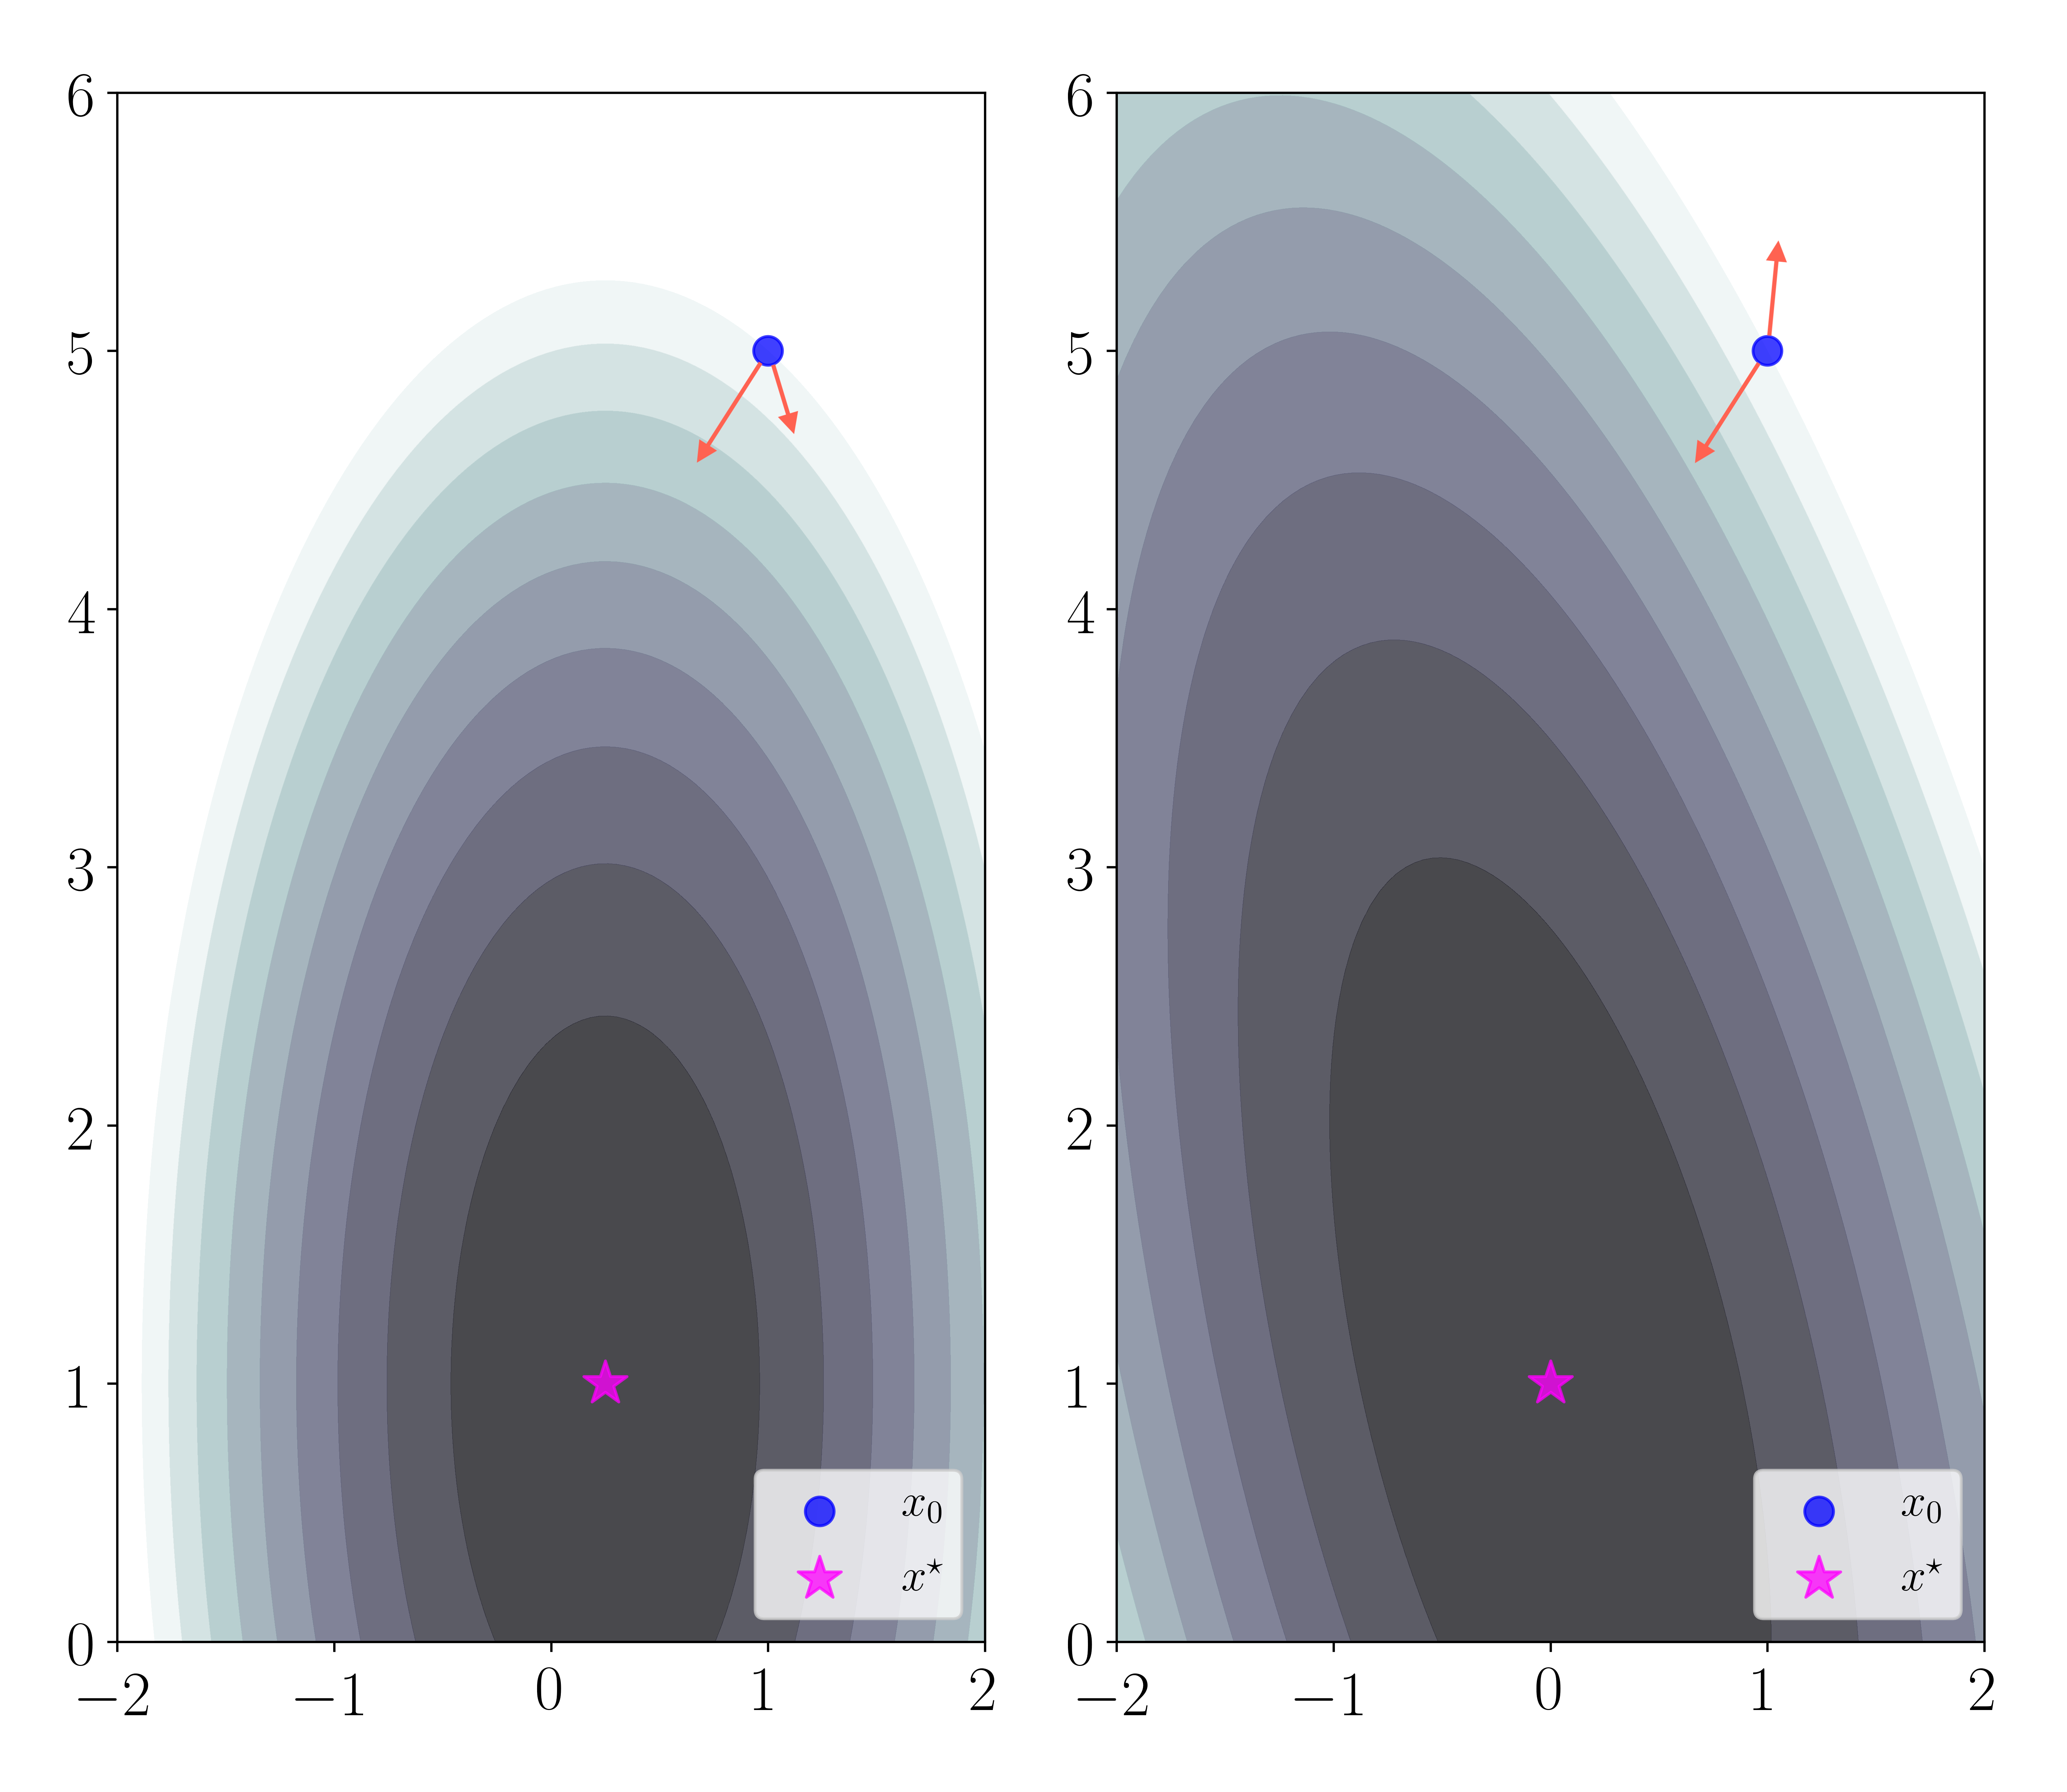
\includegraphics{figures/contours_lin-ind}}
\end{frame}
\begin{frame}
  \frametitle{first-order iterative methods}
  %
  % \pause
  \begin{block}{search direction}
    \begin{itemize}
      \item \textit{first-order methods} use current (and possibly historical) gradient information to determine the next iterate
      \item update $x_k$ with a step in direction $d_k$ with
      \begin{align}
        d_k \in x_0 + \vspan \{\nabla f(x_0), \nabla f(x_1), \nabla f(x_2), \ldots, \nabla f(x_{k})\}
      \end{align}
      \vspace{-0.15cm}
      \begin{itemize}
        \item gradient descent (GD): $d_k = -\nabla f(x_k)$
        \item steepest descent (SD): $d_k = -\nabla f(x_k)$
        \item coordinate descent (CD): $[d_k]_{i} = -[\nabla f(x_k)]_{i}$ if $i = \hat{i}$, 0 otherwise
        \item \semitransp{conjugate gradient (CG)}: tbd
      \end{itemize}
    \end{itemize}
  \end{block}
  %
  % \pause
  \begin{block}{stepsize}
    \begin{itemize}
      \item GD: $\alpha \gets \bar{\alpha} \in \mathbb{R}_+$
      \item SD: $\alpha \gets \alpha^{\star}$ where $\alpha^{\star} = \argmin_{\alpha} f(x_k + \alpha d_k)$
      \item CD: $\alpha \gets \alpha^{\star}$ where $\alpha^{\star} = \argmin_{\alpha} f(x_k + \alpha d_k)$ (different $d_k$)
      \item \semitransp{CG: tbd}
    \end{itemize}
  \end{block}
  %
\end{frame}
%
\begin{frame}
  \frametitle{quadratic example (cont'd)}
  \centering \resizebox{!}{8cm}{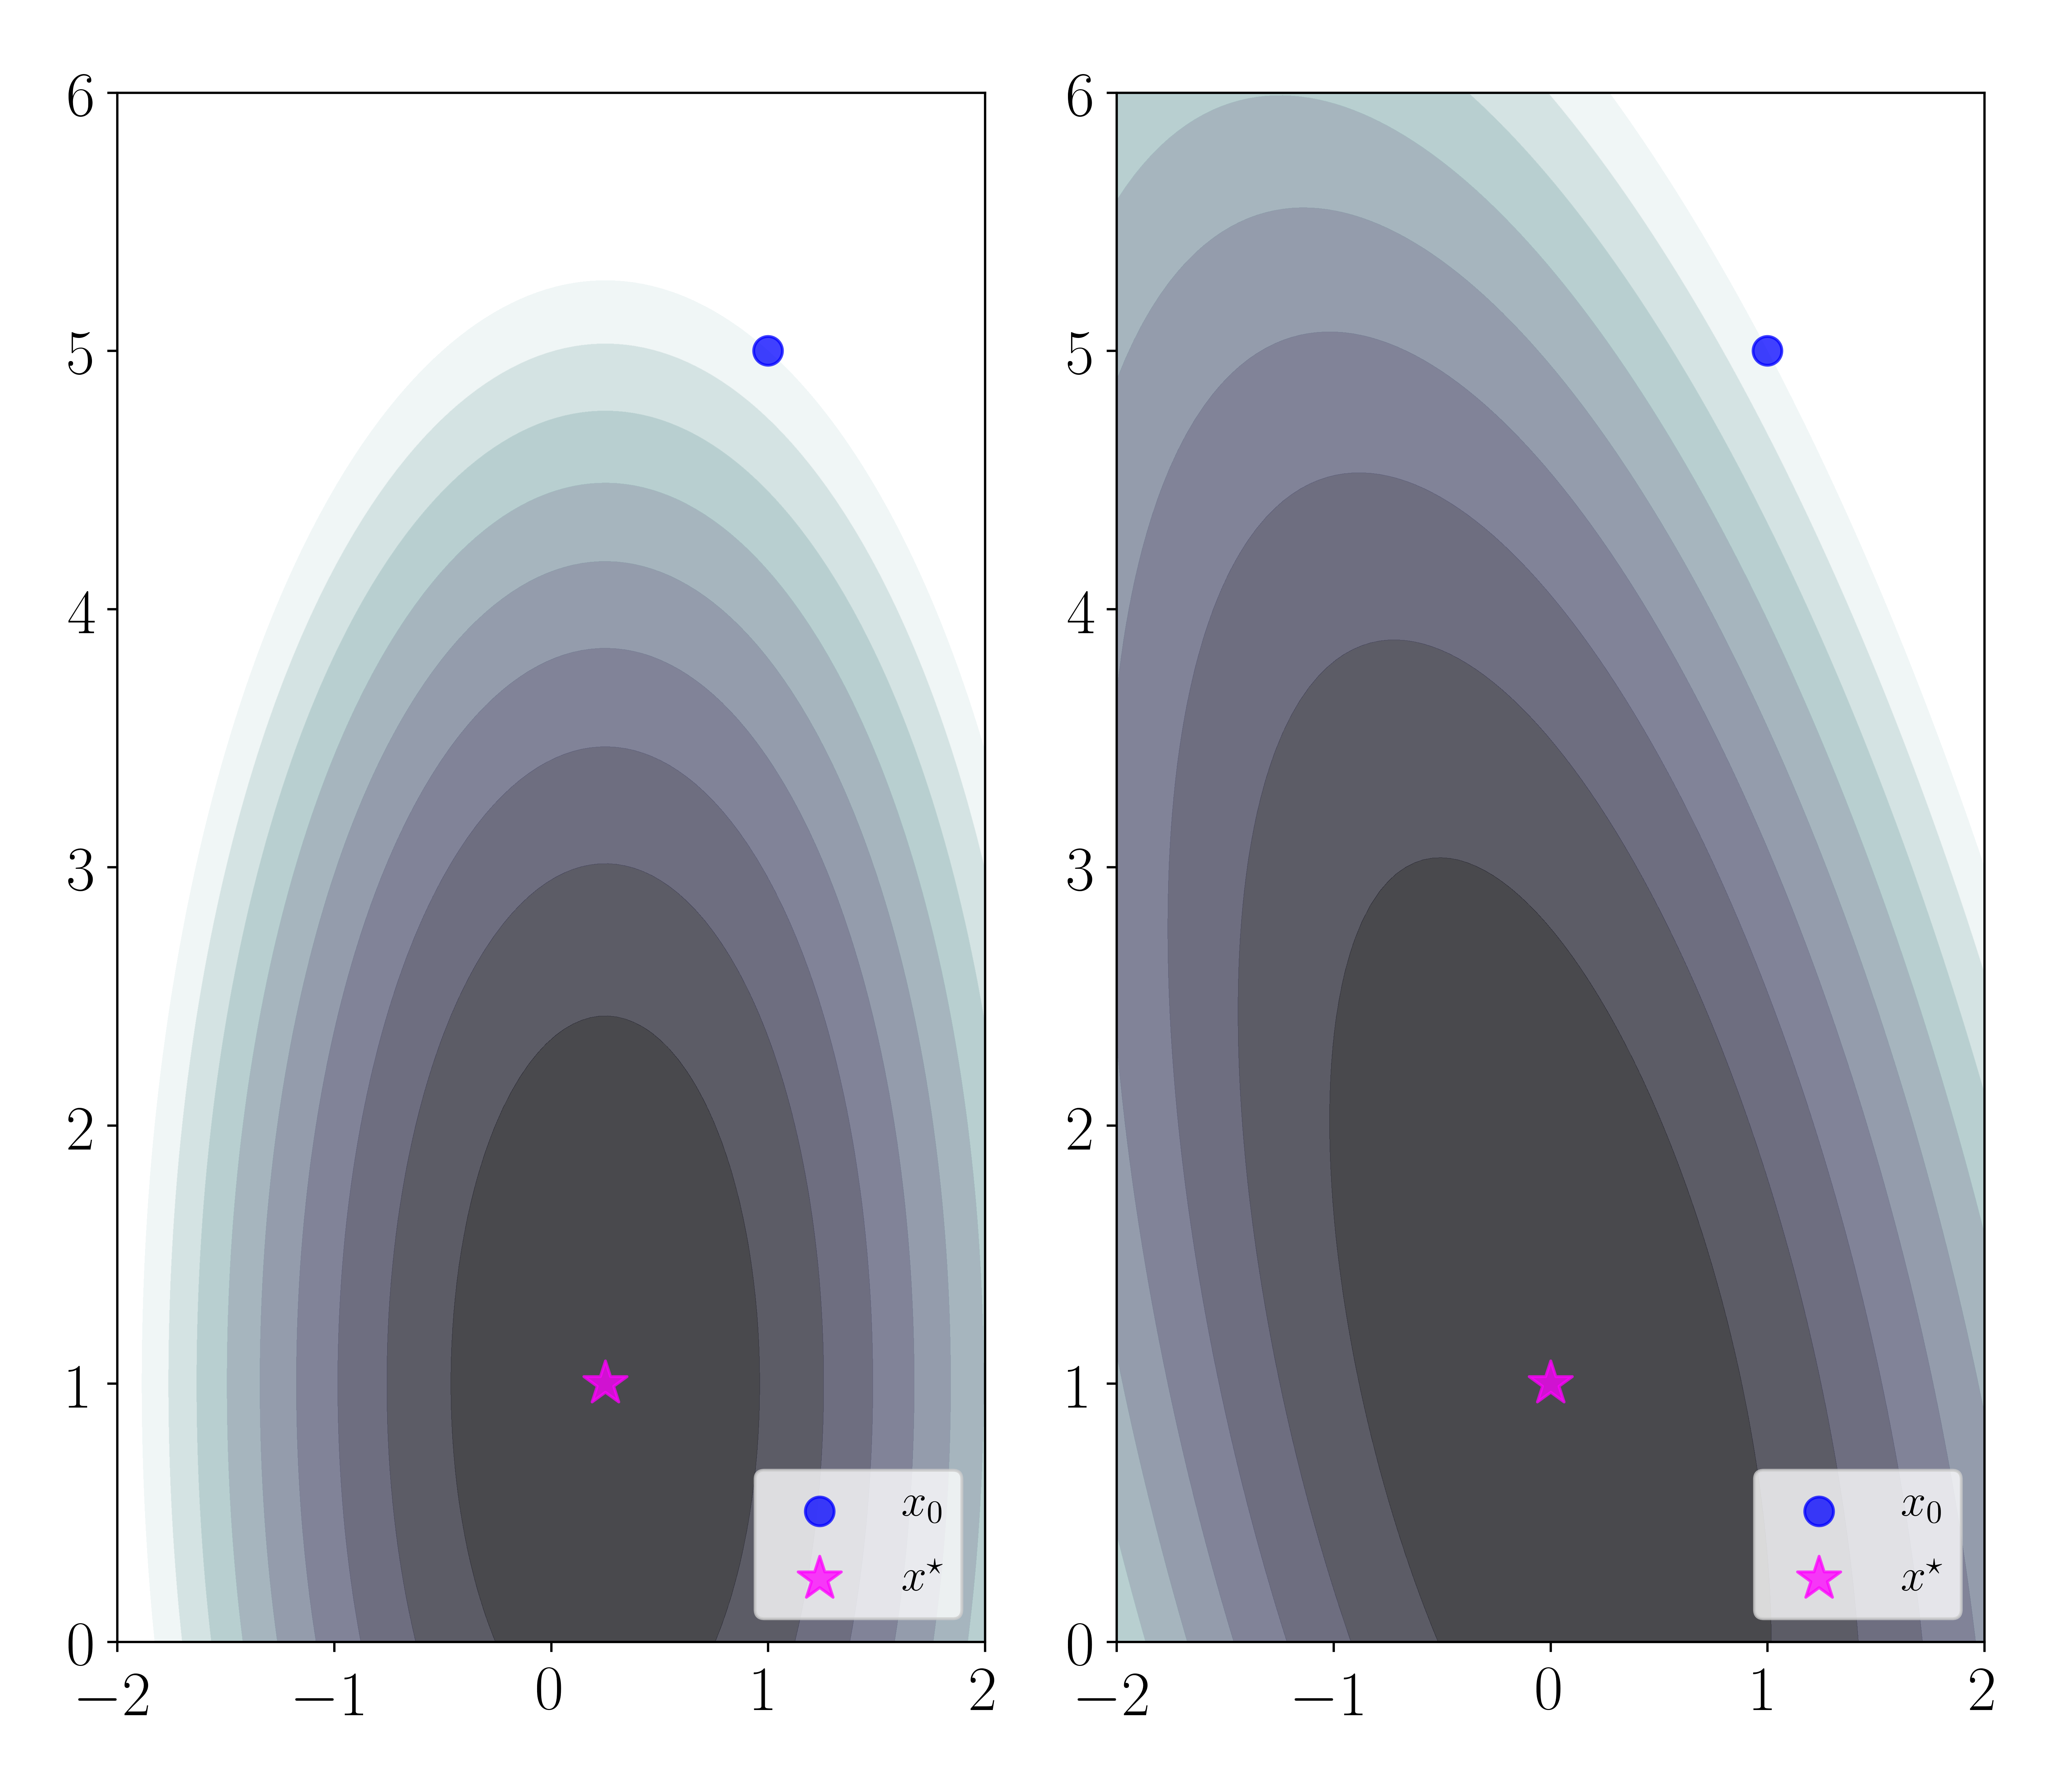
\includegraphics{figures/contours}}
\end{frame}
%
\begin{frame}
  \frametitle{quadratic example (cont'd)}
  \centering \resizebox{!}{8cm}{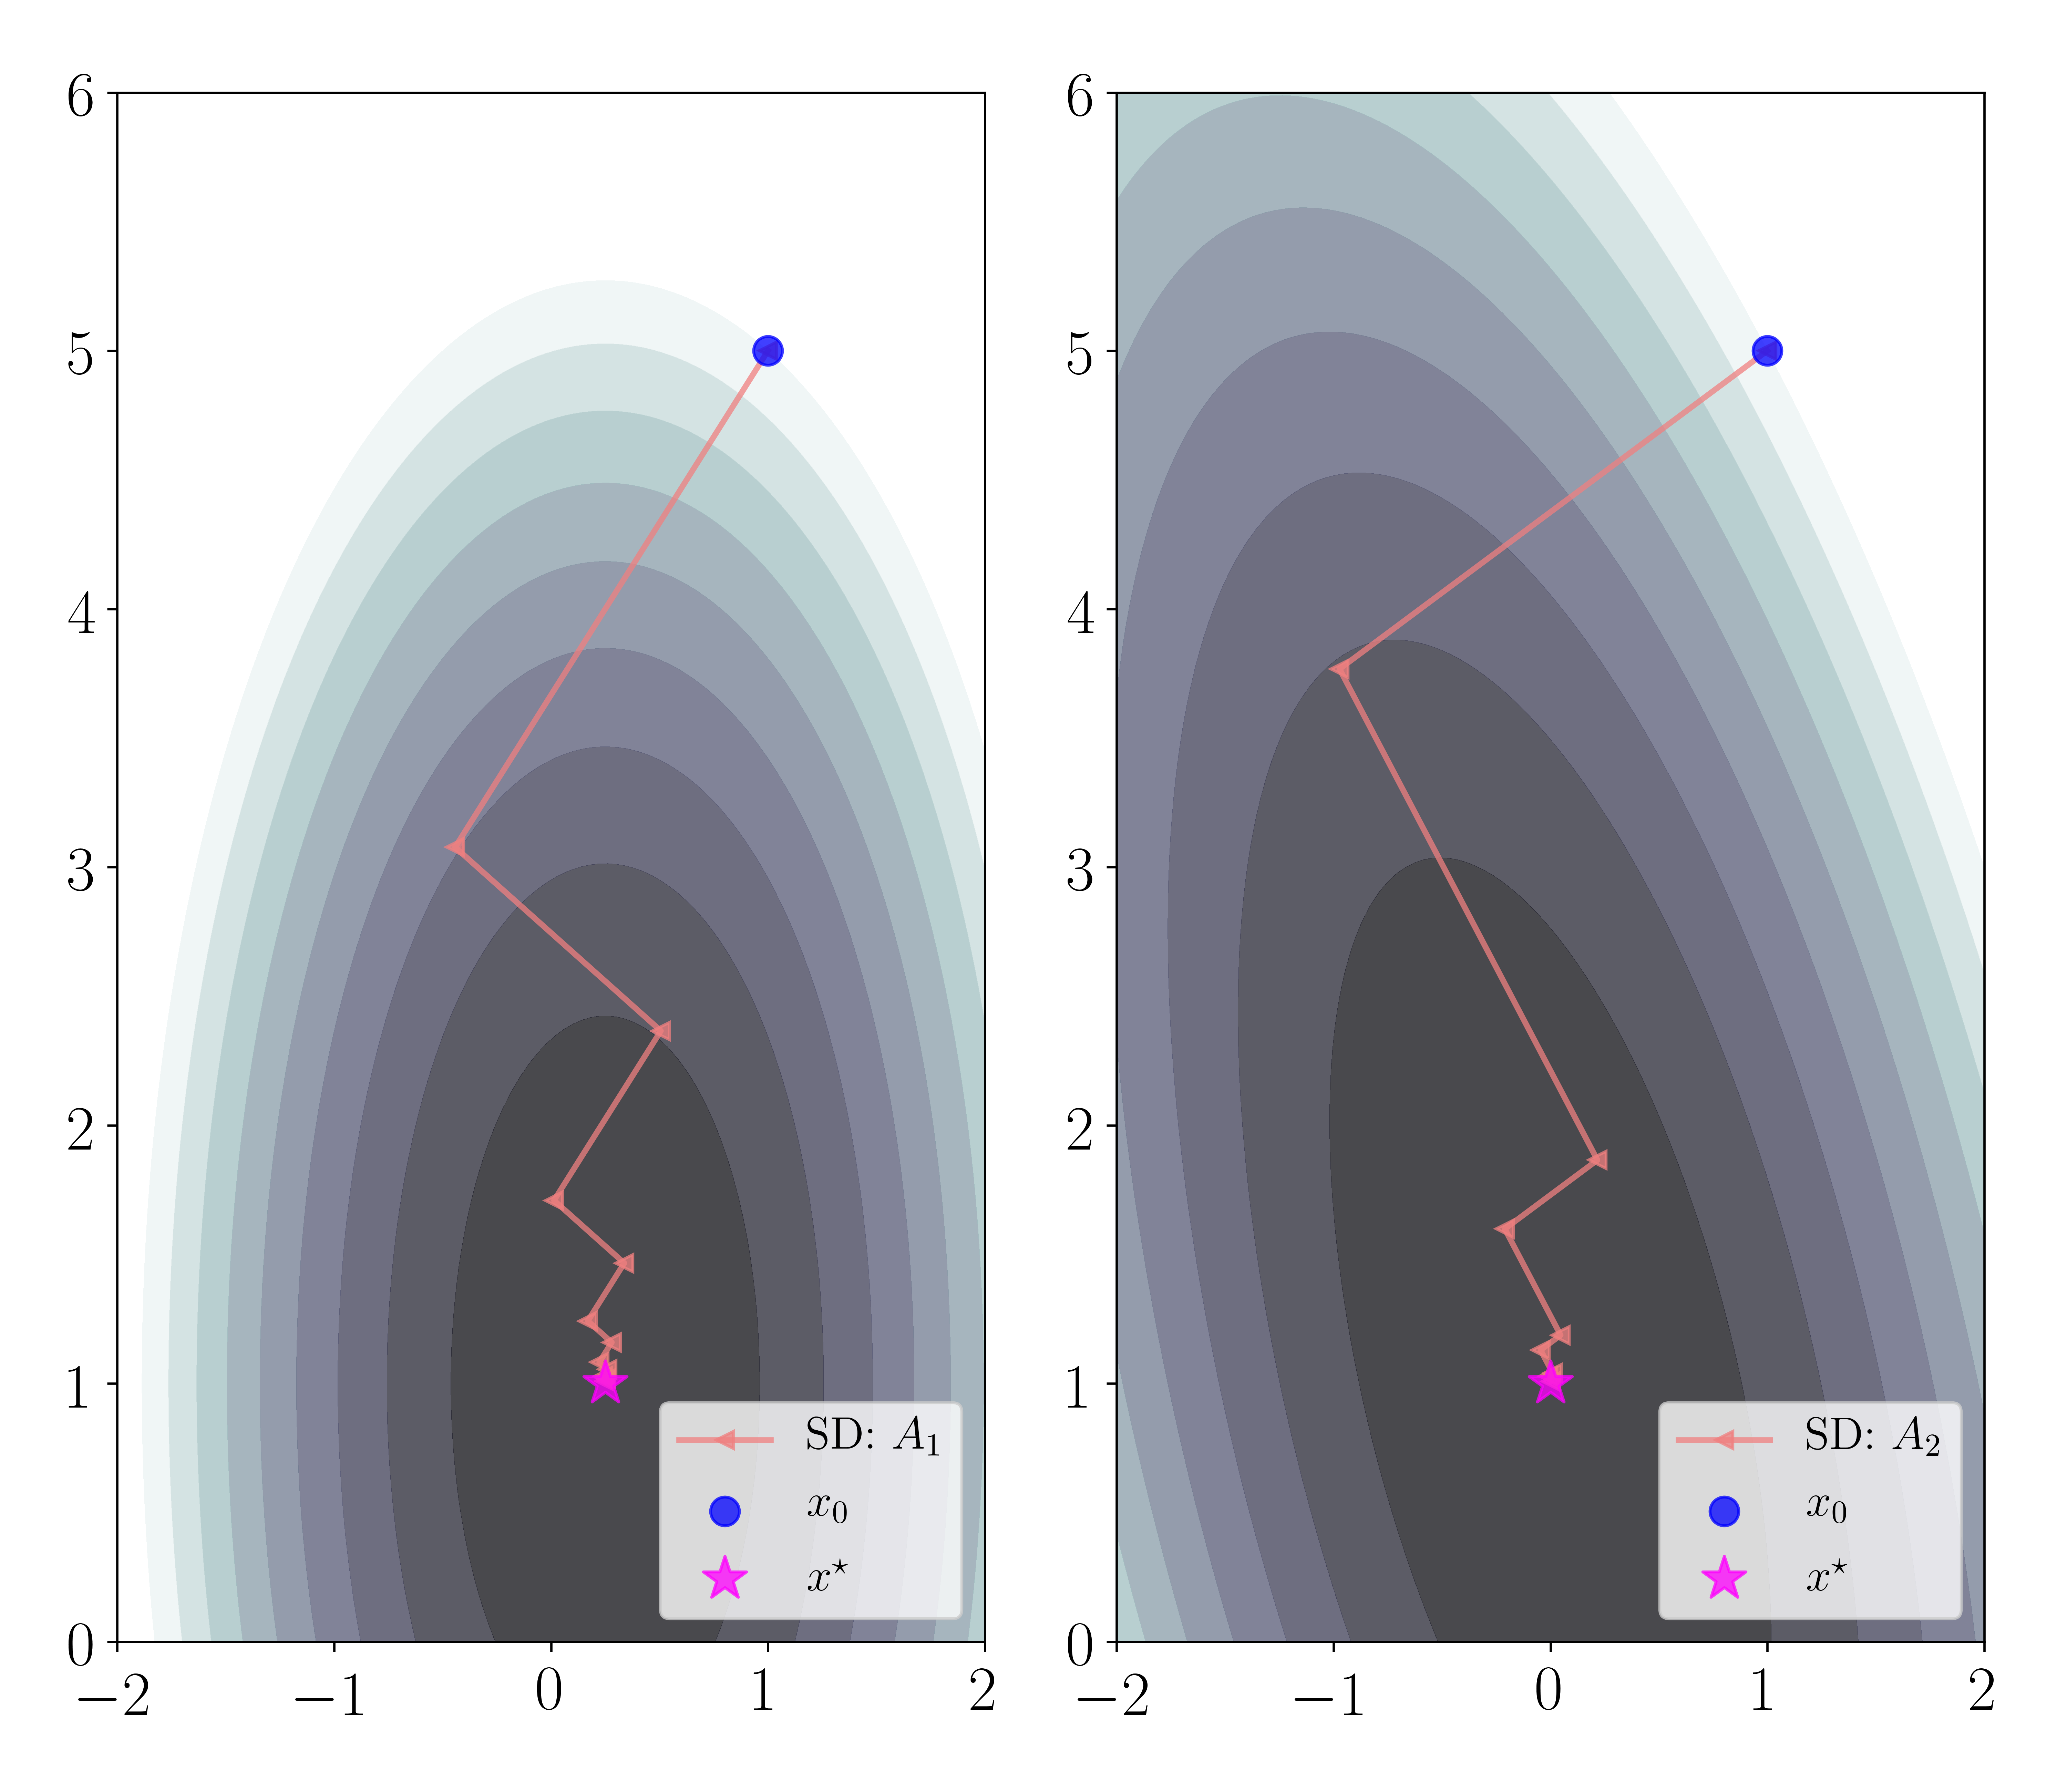
\includegraphics{figures/sd}}
\end{frame}
%
\begin{frame}
  \frametitle{quadratic example (cont'd)}
  \centering \resizebox{!}{8cm}{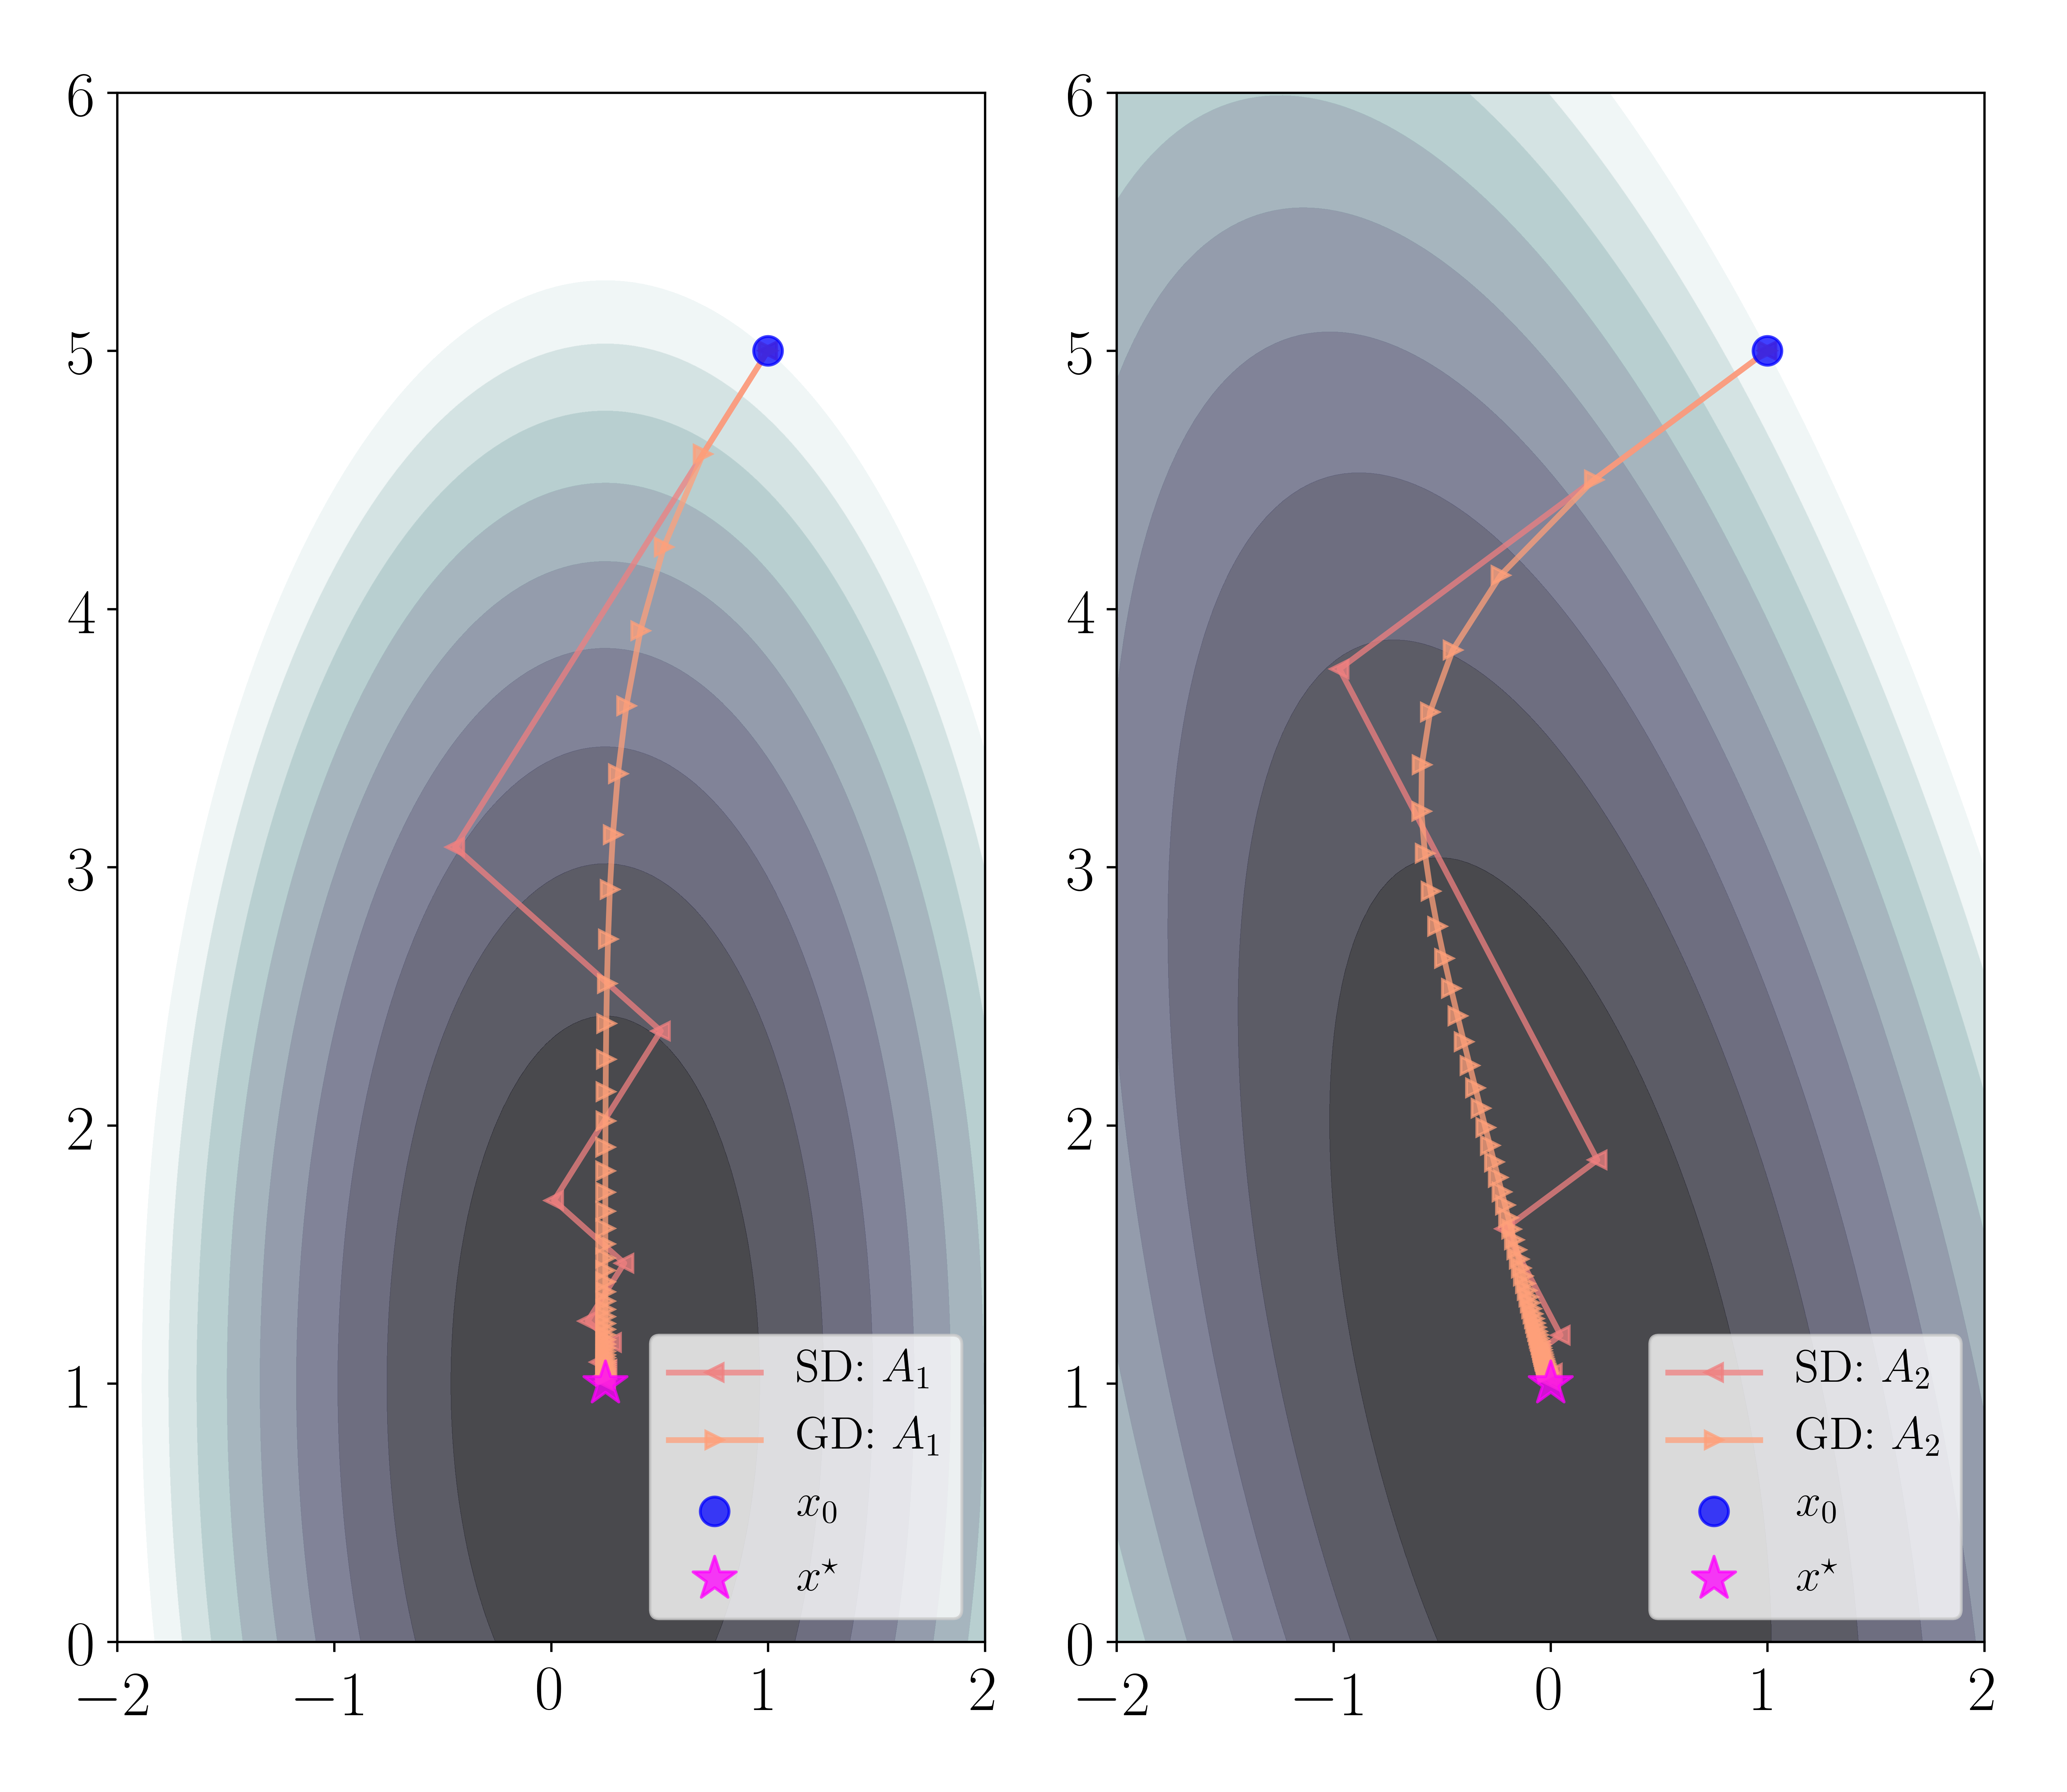
\includegraphics{figures/sd_gd}}
\end{frame}
%
\begin{frame}
  \frametitle{quadratic example (cont'd)}
  \centering \resizebox{!}{8cm}{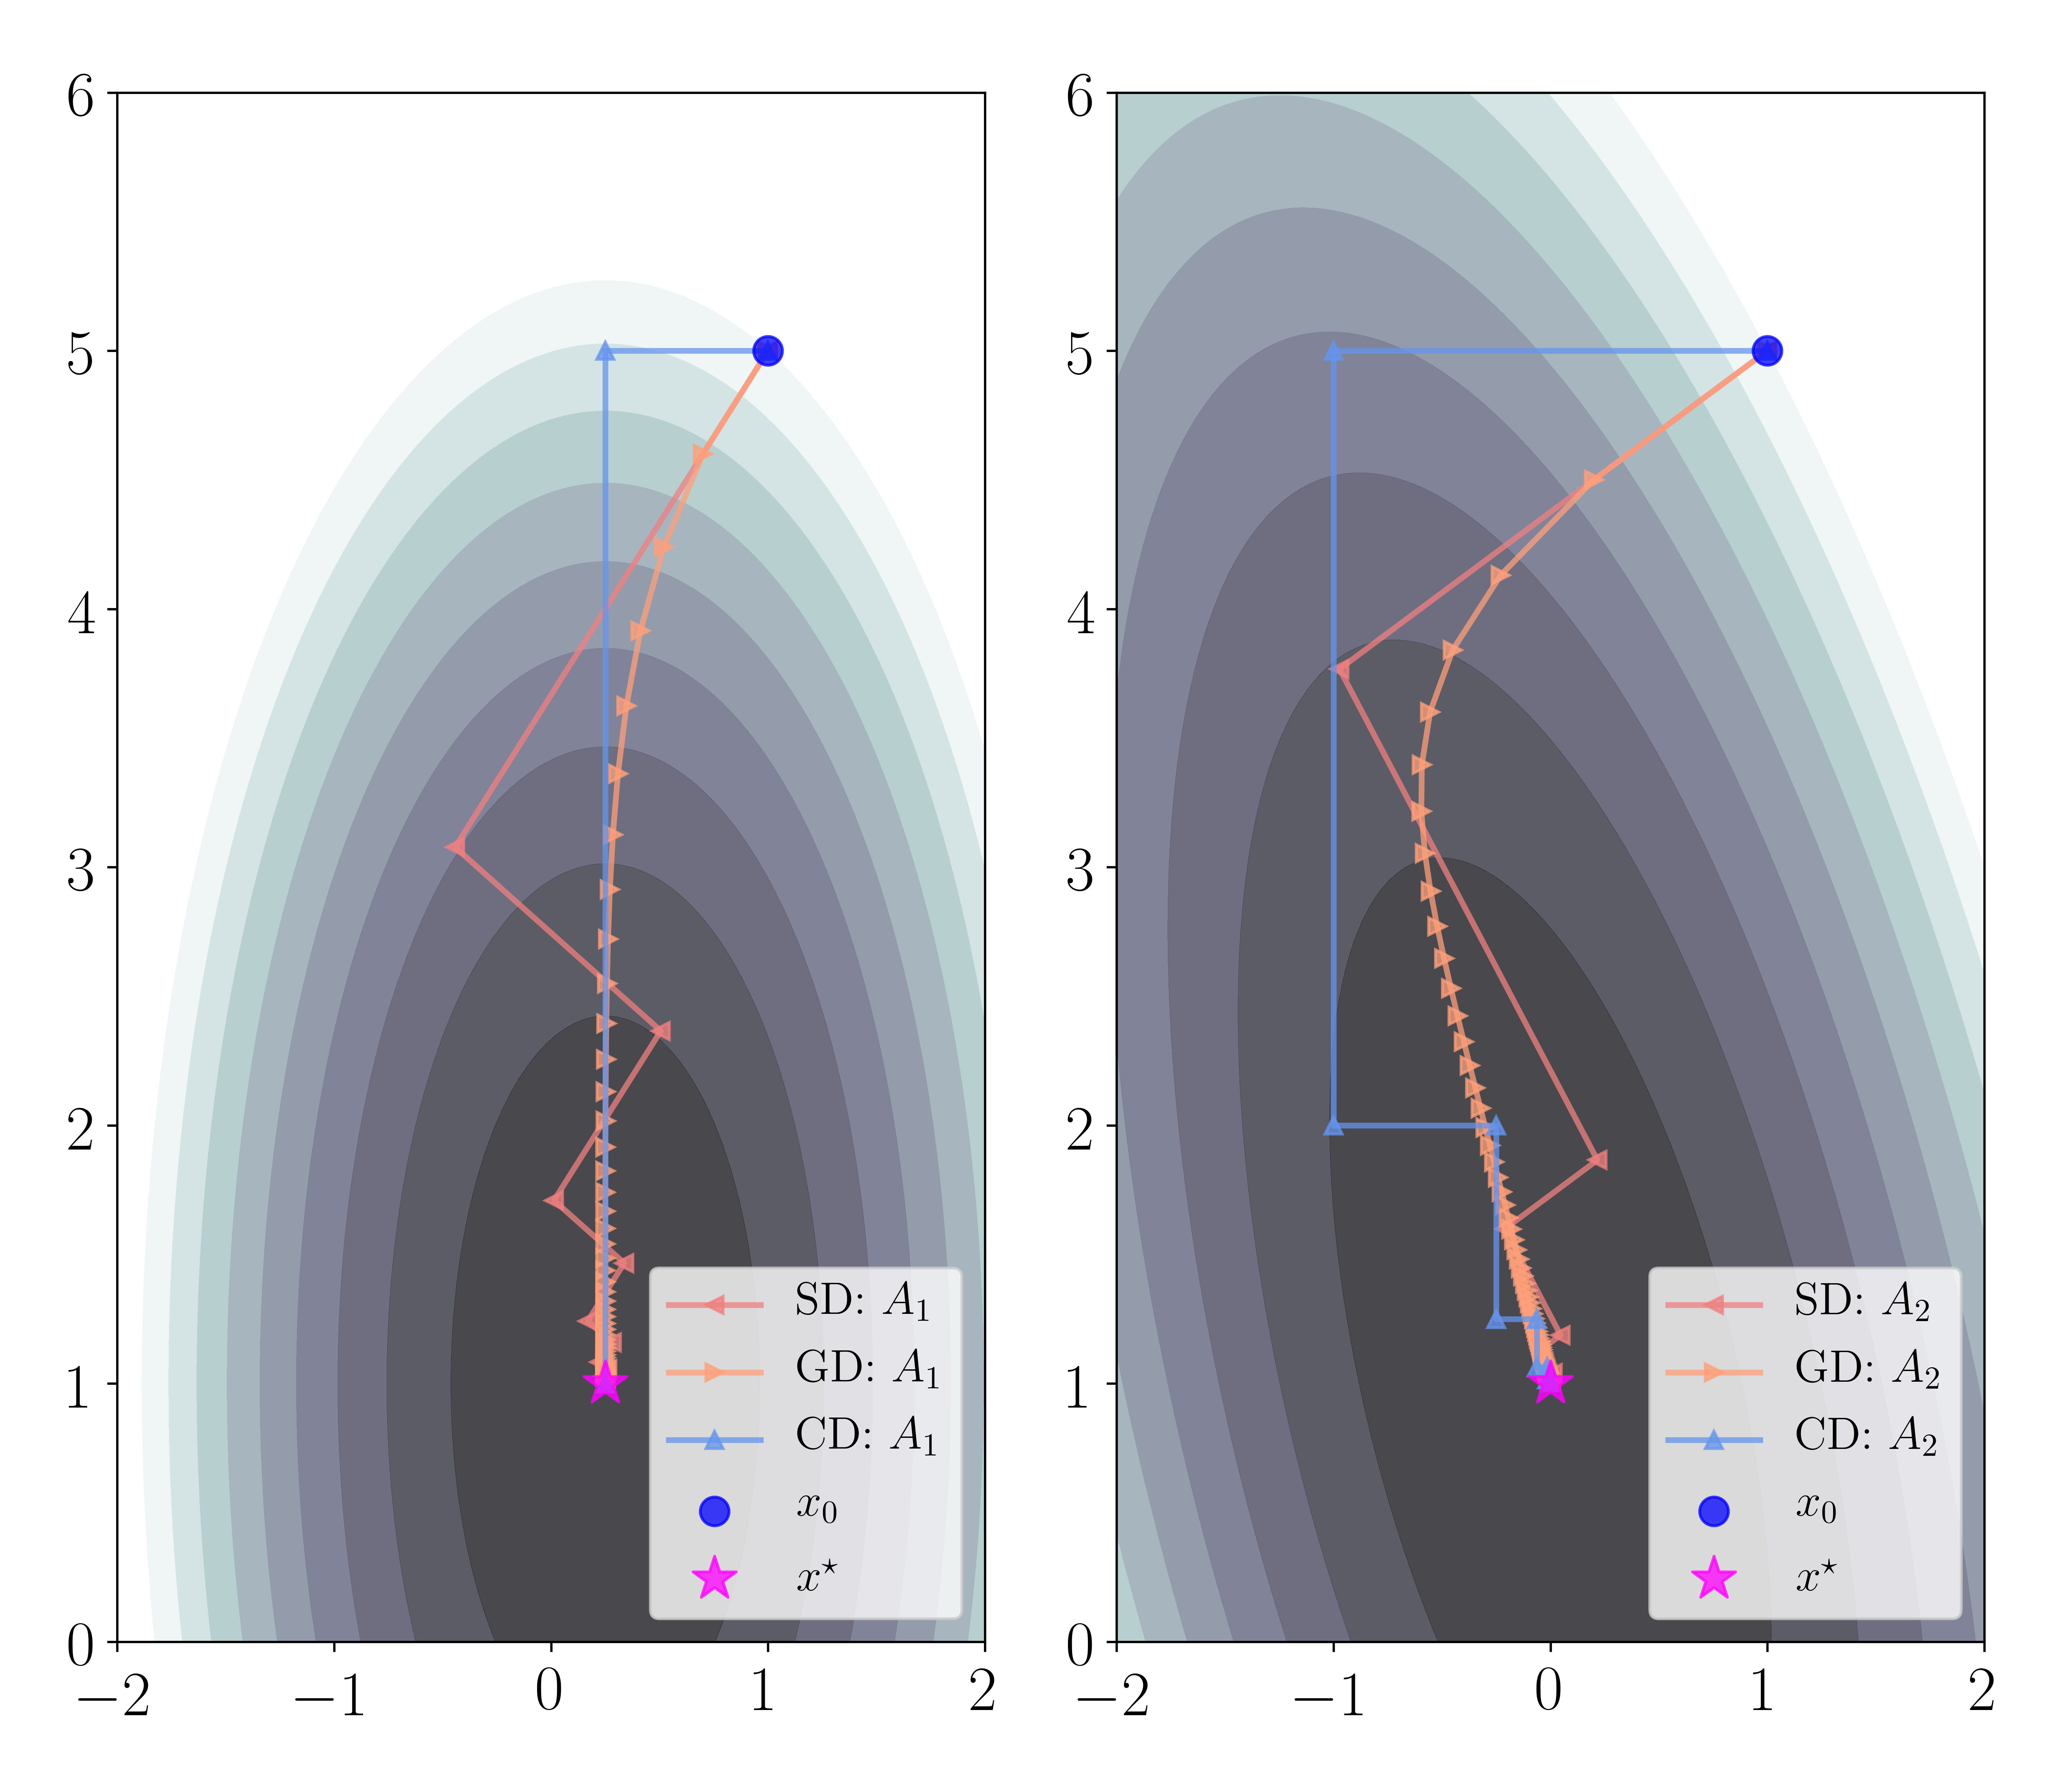
\includegraphics{figures/sd_gd_cd}}
\end{frame}
%
\begin{frame}
  \frametitle{quadratic example (cont'd)}
  \centering \resizebox{!}{8cm}{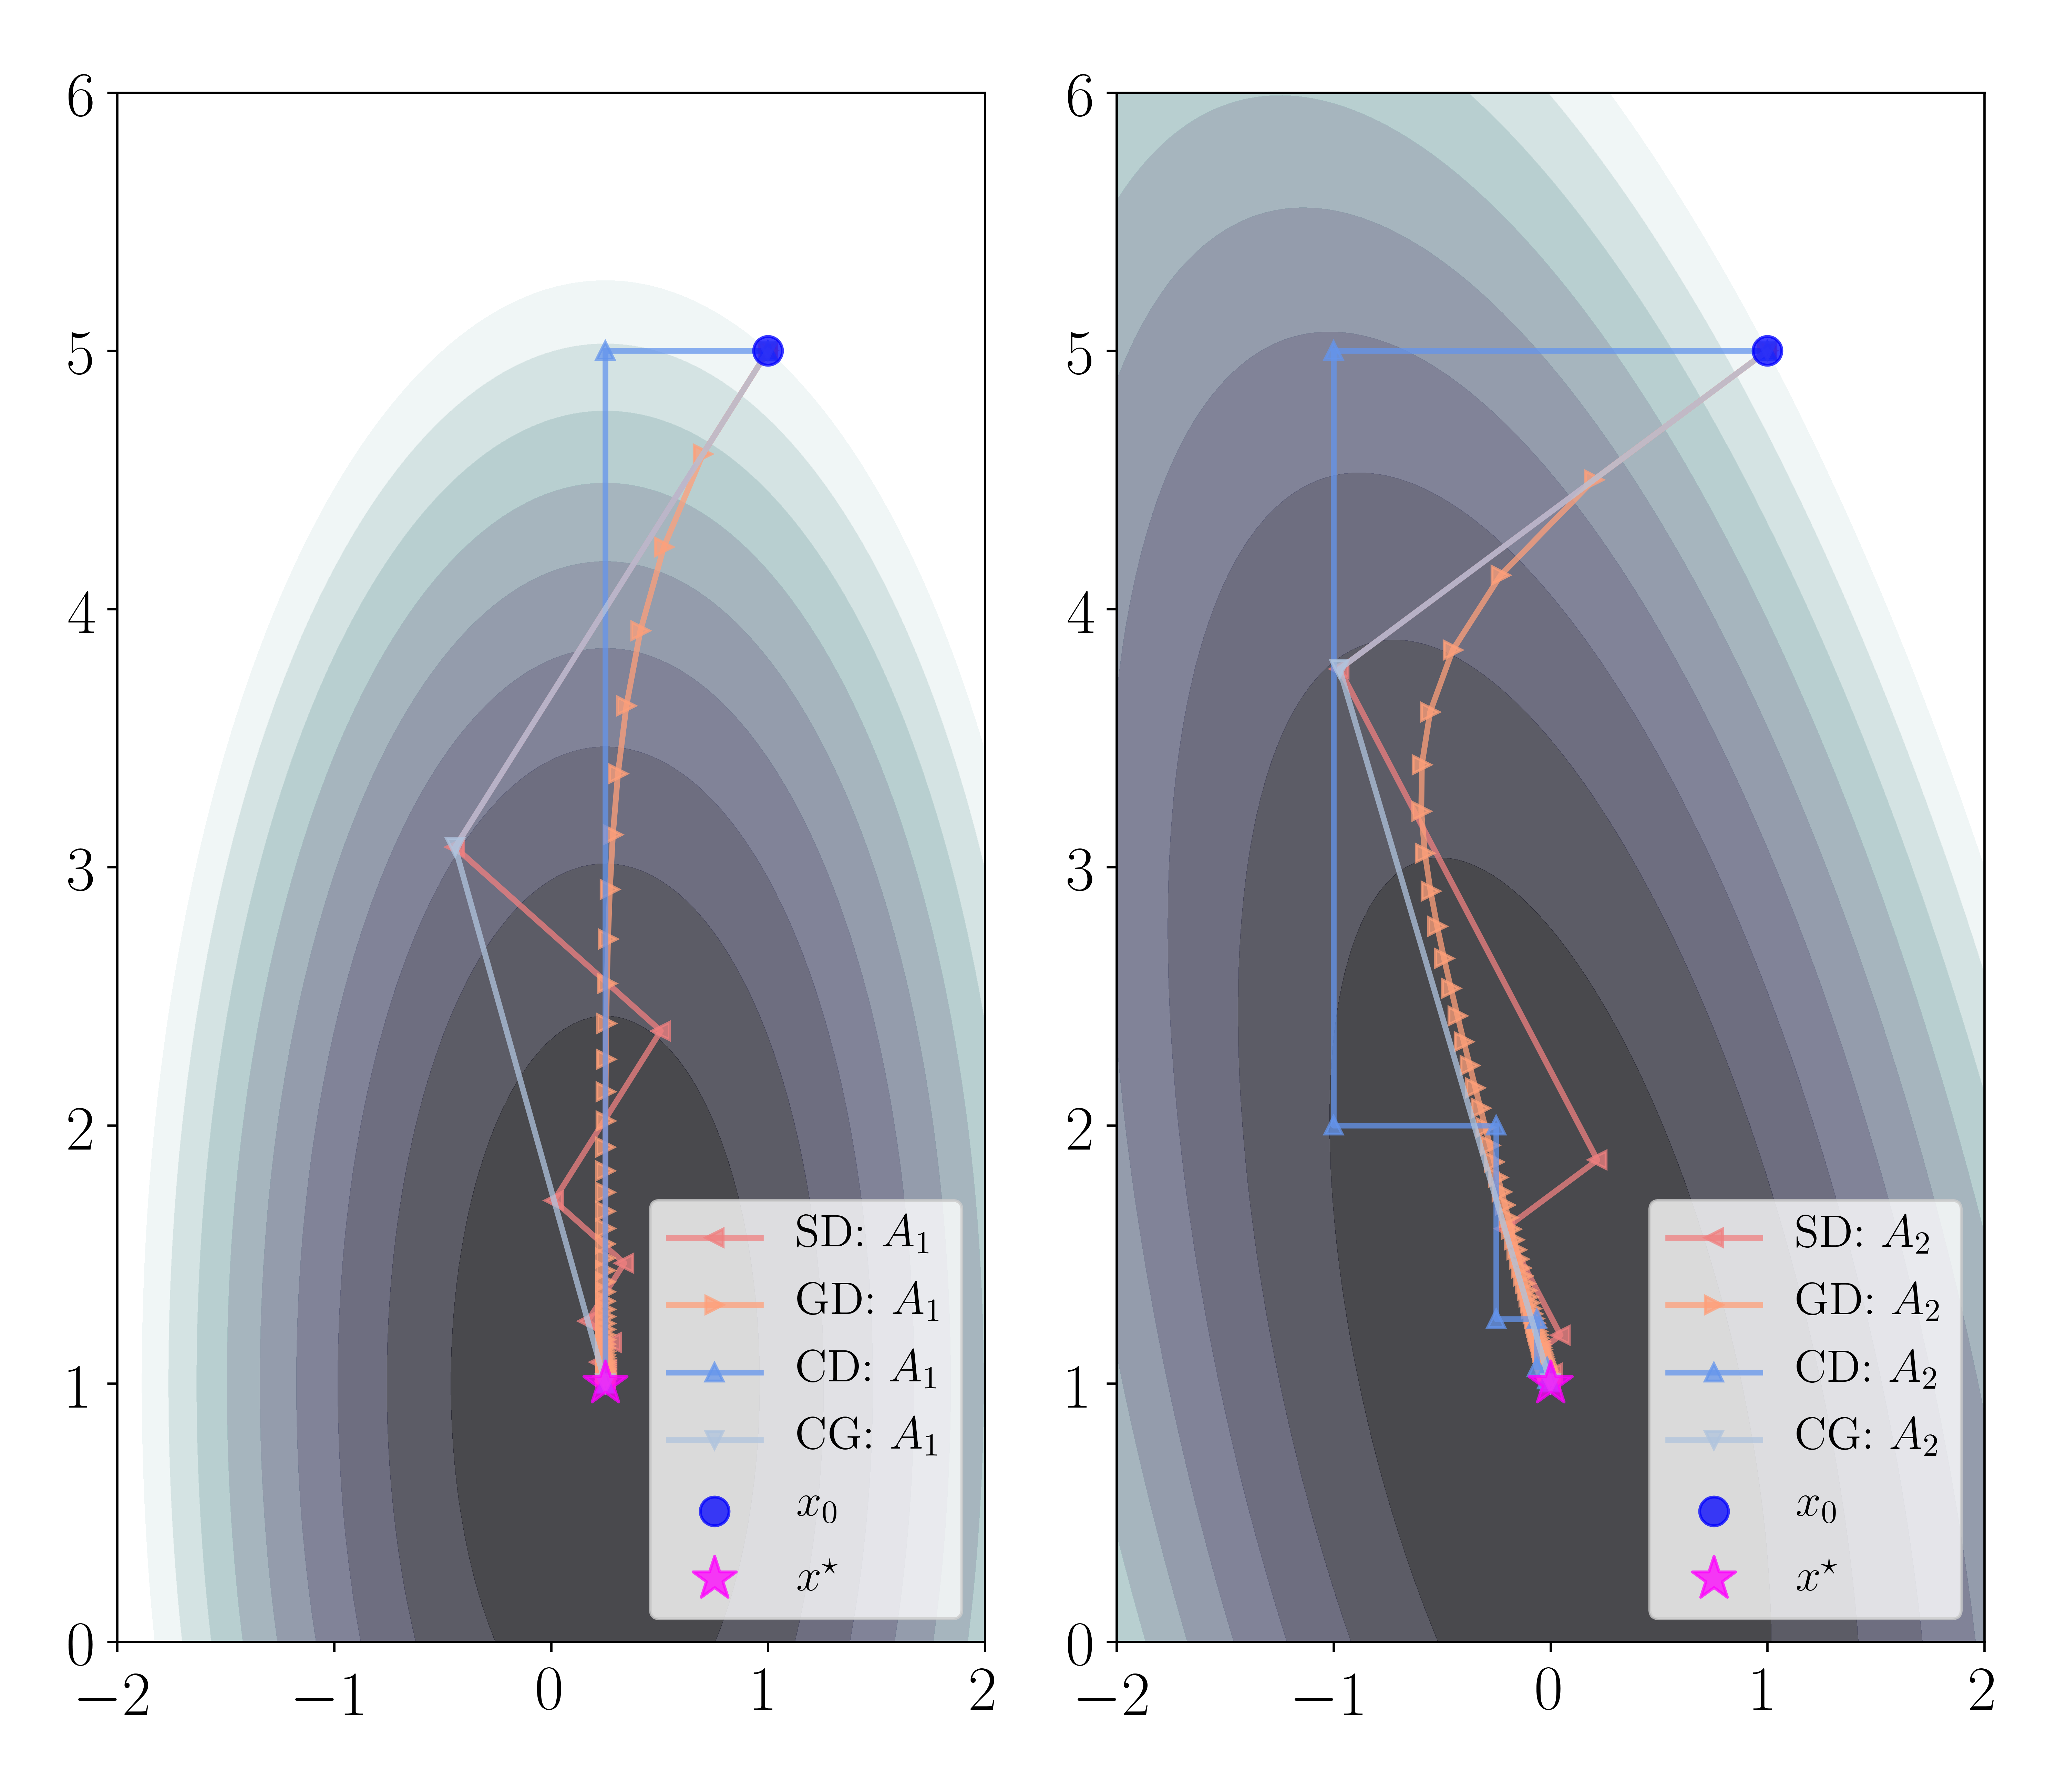
\includegraphics{figures/sd_gd_cd_cg}}
\end{frame}
%
\begin{frame}
  \frametitle{orthogonality and conjugacy}
  %
  \pause
  \begin{definition}[orthogonality]
    \label{def:orthogonal}
    a set of vectors $\{d_1, d_2, \ldots \}$ are \emph{orthogonal}, that is $d_i \perp d_j$, if $\langle d_i,\, d_j \rangle = 0$ for $i \ne j$
  \end{definition}
  %
  \pause
  \begin{definition}[conjugacy]
    \label{def:conjugate}
    a set of vectors $\{d_1, d_2, \ldots \}$ are \emph{conjugate} (orthogonal in a geometry induced by some $A \succ 0, A=A^{\top}$) if $ \langle d_i,\, d_j \rangle_A \coloneqq \langle d_i,\, A d_j \rangle = 0$ for $i \ne j$
  \end{definition}
  %
  \pause
  \centering \resizebox{!}{4cm}{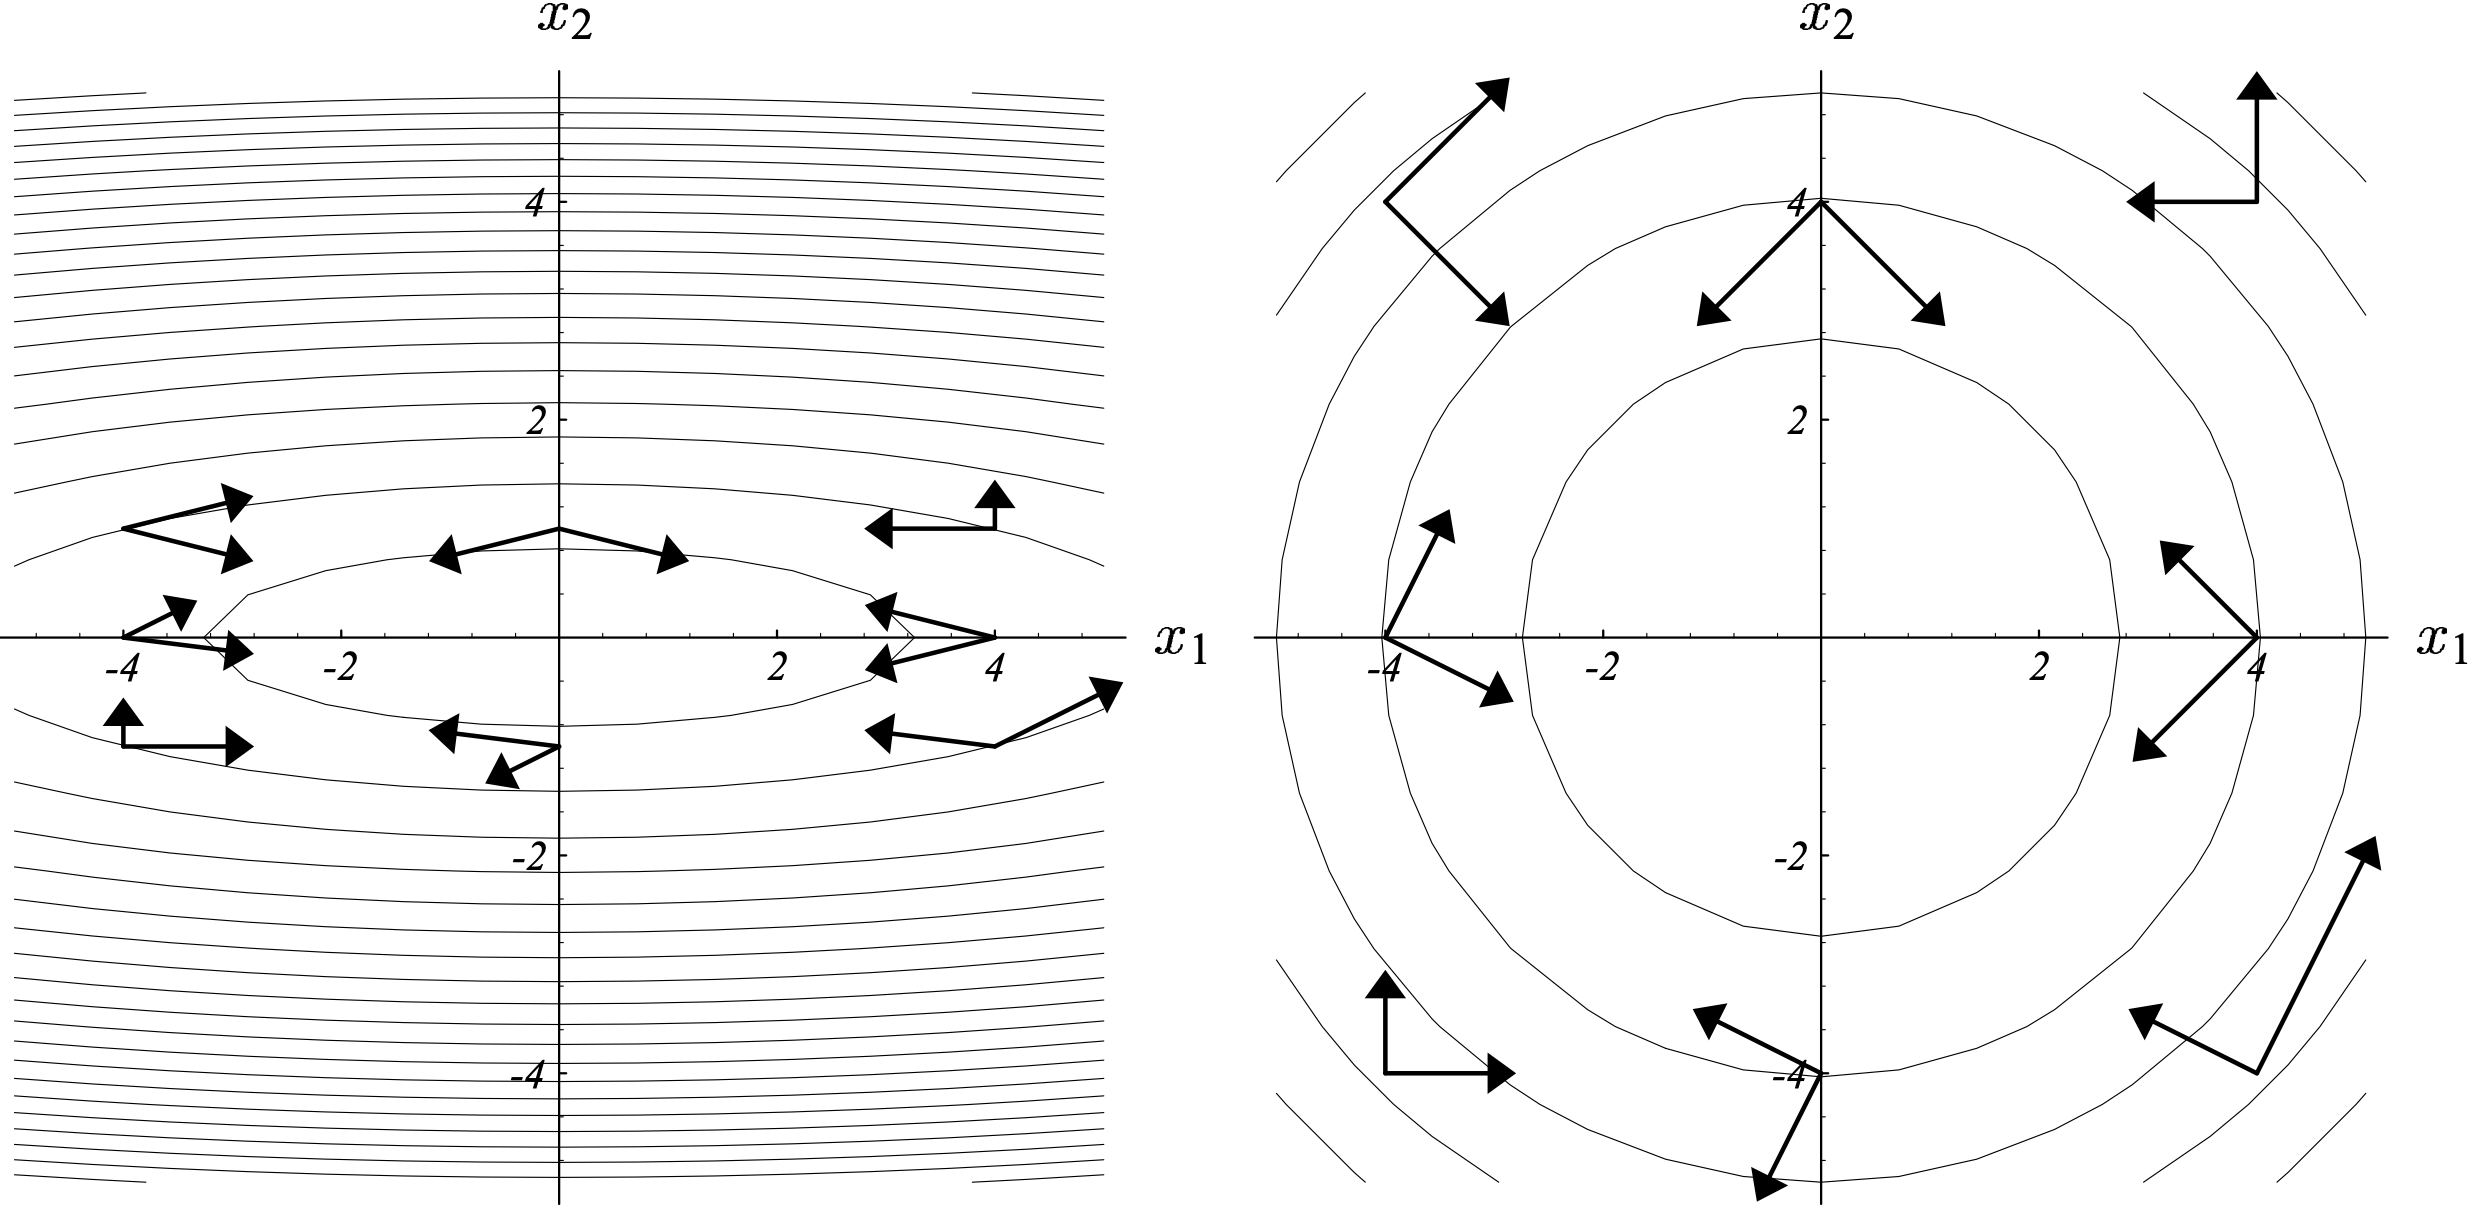
\includegraphics{figures/conjugate}}\cite{shewchuk_cg_1994}
  %
\end{frame}
%
\begin{frame}
  \frametitle{revisting coordinate descent (diagonal)}
  %
  \pause
  \begin{assumption*}
    $A$ is diagonal and $D = [d_0,\, d_1,\, \ldots,\, d_{n-1}] \in \mathbb{R}^{n \times n}$ contains $n$ orthogonal directions; note that the principal axes of $f$'s contours will align with $d_i$
  \end{assumption*}
  %
  \pause
  \begin{alertblock}{reconstruct the error}
    %
    define error $e \coloneqq D \alpha$ with $\alpha = [\alpha_0,\, \ldots,\, \alpha_{n-1}]^{\top}$,
    %
    \begin{align}
      \hspace{-2\leftmargin}
      \label{eq:split-function-scalar}
      f(x + e) &= f(x) + \sum_{i,j} x_i A_{i,j} e_j + \tfrac 12 \sum_{i,j} d_i A_{i,j} e_j - \sum_i b_i e_i \\
      \begin{split}
        &= f(x) + \sum_{i,j} x_i A_{i,j} \sum_k \alpha_k d_{k,j} \\
        &\qquad + \tfrac 12 \sum_{i,j} \sum_k \alpha_k d_{k,i} A_{i,j}\sum_k \alpha_k d_{k,j} - \sum_i b_i \sum_k \alpha_k d_{k,i}
      \end{split}
      \\
      &= f(x) + \sum_k \left[ \tfrac 12 \alpha_k^2 d_k^{\top} A d_k + \alpha_k x^{\top} A d_k - \alpha_k b^{\top} d_k \right]
    \end{align}
    %
    so finally $\min_{\alpha} f(x + e) = f(x) + \sum_{k=0}^{n-1} \left\{ \min_{\alpha_k} f(\alpha_k d_k) \right\}$
  \end{alertblock}
  %
\end{frame}
%
\begin{frame}
  \frametitle{revisiting coordinate descent (non-diagonal, I)}
  %
  \pause
  \begin{assumption*}
    suppose that $D$ contains $n$ $A$-conjugate vectors
  \end{assumption*}
  %
  \pause
  \begin{alertblock}{interpretation 1: coordinate descent in $D^{-1}$ space}
    %
    \begin{itemize}
      \item how can we convert to the diagonal case?
      \pause
      \begin{itemize}
        \item change coordinates so that $\hat{x} = D^{-1}x$, and rewrite \cref{eq:quadratic-program}
      \end{itemize}
      %
      \begin{align}
        \label{eq:quadratic-program-coordinate}
        f(\hat{x}) = \tfrac 12 \hat{x}^{\top} (D^{\top} A D) \hat{x} - (D^{\top}b)^{\top} \hat{x}
      \end{align}
      %
      \item \pause by conjugacy, $D^{\top} A D$ is diagonal!
      \item \pause proceed by solving $n$ 1-dimensional minimization problems along each coordinate direction of $\hat{x}$ \cite{nocedal_numerical_2006}
    \end{itemize}
    %
  \end{alertblock}
  %
\end{frame}
%
\begin{frame}
  \frametitle{revisiting coordinate descent (non-diagonal, II)}
  %
  \pause
  \begin{assumption*}
    suppose that $D$ contains $n$ $A$-conjugate vectors
  \end{assumption*}
  %
  \pause
  \begin{alertblock}{interpretation 2: line search simplification}
    %
    \begin{itemize}
      \item rewrite \cref{eq:split-function-scalar} in vector form as
      %
      \begin{align}
        \label{eq:split-function-vector}
        f(x + e) &= f(x) + \tfrac 12 \alpha^{\top} D^{\top} A D \alpha + (D\alpha)^{\top} (Ax) - (D\alpha)^{\top} b \\
        &= f(x) + \tfrac 12 \alpha^{\top} D^{\top} A D \alpha + (D\alpha)^{\top} (Ax - b)
      \end{align}
      %
      so that $\alpha^{\star} = \argmin_{\alpha} f(x + D\alpha)$ satisfies
      %
      \begin{align}
        \label{eq:split-minimization-vector}
        \alpha^{\star} = (D^{\top} A D)^{-1} D^{\top} (Ax-b)
      \end{align}
      %
    \end{itemize}
    %
  \end{alertblock}
  %
\end{frame}
%
\begin{frame}
  \frametitle{revisiting coordinate descent (non-diagonal, III)}
  %
  \begin{block}{takeaway: $k$-optimality}
    \begin{itemize}
      \item define the subspace $M_k \coloneqq x_0 + \vspan \{ d_0, d_1, \ldots, d_{k} \}$
      \item after $k$ steps, we have minimized the error \emph{as much as possible} in the subspace $M_k \subset \mathbb{R}^n$
      \item $x_k = \argmin_{x \in M_k} f(x)$
      \item hence gradients $\nabla_x f(x_{k+i}) \perp M_k$ for $i > 0$
      \begin{itemize}
        \item $x_k$ is optimal, so directional derivative is zero
        \item $\langle \nabla_x f(x_k),\, v \rangle = 0, \quad \forall v \in M_k$
      \end{itemize}
    \end{itemize}
  \end{block}
  %
\end{frame}
%
\section{Computation}% linear algebra
\label{sec:computation}
%
\begin{frame}
  \frametitle{getting conjugate directions}
  %
  \pause
  \begin{block}{modify Gram-Schmidt process for orthogonality wrt $A$}
    \begin{itemize}
      \item start with gradients $g_k \coloneqq \nabla_x f(x_k)$ at each step as the orthogonalization vectors
      % \item define the subspace $M_k = x_0 + \vspan \{ d_0, d_1, \ldots, d_{k} \}$
      %
      \begin{align}
        \label{eq:A-conjugate}
        d_{k+1} = g_{k+1} - \mathrm{proj}_{M_k}\,(g_{k+1}) = g_{k+1} - \sum_{i=0}^k \frac{\left\langle g_{k+1},\, d_j \right\rangle_A} {\left\langle d_j,\, d_j \right\rangle_A} \, d_j
      \end{align}
      %
      \item computationally intensive and G-S is not numerically stable
    \end{itemize}
    %
  \end{block}
  %
  \pause
  \begin{block}{goal}
    simplify $\mathrm{proj}_{M_k}\,(g_{k+1})$ as much as possible \cite{zibulevsky_lectures}
  \end{block}
\end{frame}
%
\begin{frame}
  \frametitle{conjugate gradients procedure (simplification I)}
  %
  \begin{block}{simplification I: projection summation}
    \begin{enumerate}
      \item \pause solve for $d_k$ in terms of the quantities $x_k, x_{k+1}, \alpha_k$ so
      %
      \begin{align}
        d_k = \frac{1}{\alpha_k} (x_{k+1} - x_k)
      \end{align}
      %
      \item \pause multiply by $A$ (and cancel $b$ terms)
      %
      \begin{align}
        A d_k = \frac{1}{\alpha_k} A (x_{k+1} - x_k) = \frac{1}{\alpha_k} A (g_{k+1} - g_k)
      \end{align}
      %
      \item \pause use $k$-optimality
      \begin{itemize}
        \item orthogonality of gradients $g_{k+1} \perp M_k \implies g_{k+1} \perp \{ g_0, g_1, \ldots, g_{k} \}$ since $\vspan \{ g_0, g_1, \ldots, g_{k} \} = M_k$ (taking $d_0 = g_0$)
      \end{itemize}
      \item \pause conclude
      \begin{align}
        d_{k+1} = g_{k+1} - \frac{\langle g_{k+1}, (g_{k+1} - g_k) \rangle} {\langle d_k, (g_{k+1} - g_k \rangle} d_k = \beta_k d_k
      \end{align}
    \end{enumerate}
  \end{block}
  %
\end{frame}
%
\begin{frame}
  \frametitle{conjugate gradients procedure (simplification II)}
  %
  \begin{block}{simplification II: $\beta_k$}
    \begin{enumerate}
      \item \pause $g_{k+1} \perp d_k$ and $g_{k+1} \perp g_k$ by $k$-optimality so that
      %
      \begin{align}
        \beta_k = \frac{\langle g_{k+1}, g_{k+1} \rangle} {\langle d_k, g_k \rangle}
      \end{align}
      %
      \item \pause expand $d_k = g_k - \beta_{k-1} d_{k-1}$ and $d_k \perp g_{k-1}$ by $k$-optimality so that
      \begin{align}
        \beta_k = \frac{\langle g_{k+1}, g_{k+1} \rangle} {\langle g_k, g_k \rangle}
      \end{align}
    \end{enumerate}
  \end{block}
  %
\end{frame}
%
\begin{frame}
  \frametitle{conjugate gradients procedure}
  %
  \vspace{-0.25cm}
  \begin{align*}
    & {g}_0 \gets {A x}_0 - b;\quad {d}_0 \gets -{g}_0; \quad k \gets 0 \\
    & \text{repeat} \\
    & \qquad \alpha_k \gets \frac{{g}_k^\mathsf{T} {g}_k}{{d}_k^\mathsf{T} {A d}_k}  \\
    & \qquad {x}_{k+1} \gets {x}_k + \alpha_k {d}_k \\
    & \qquad {g}_{k+1} \gets {g}_k - \alpha_k {A d}_k \\
    & \qquad \hbox{if } {g}_{k+1} \leq \text{tolerance, then exit, else} \\
    & \qquad \beta_k \gets \frac{{g}_{k+1}^\mathsf{T} {g}_{k+1}}{{g}_k^\mathsf{T} {g}_k} \\
    & \qquad {d}_{k+1} \gets -{g}_{k+1} + \beta_k {d}_k \\
    & \qquad k \gets k + 1 \\
    & \text{end repeat} \\
    & \text{return } {x}_{k+1}
  \end{align*}
  %
  \cite{wikipedia_cg}
  %
\end{frame}
%
\section{Error (convergence) analysis}
\label{sec:error-analysis}
%
\begin{frame}
  \frametitle{NOPE!}
  but nice connections to finding roots of polynomials
\end{frame}
%
% \begin{frame}
%   \frametitle{Gradient descent}
% \end{frame}
% %
% \begin{frame}
%   \frametitle{Steepest descent}
% \end{frame}
% %
% \begin{frame}
%   \frametitle{Conjugate gradients}
%
% \end{frame}
%
\section{Application}
\label{sec:application}
%
\begin{frame}
  \frametitle{simulating tropical cyclones \cite{plotkin_maximizing_2019}}
  %
  \centering \resizebox{!}{8cm}{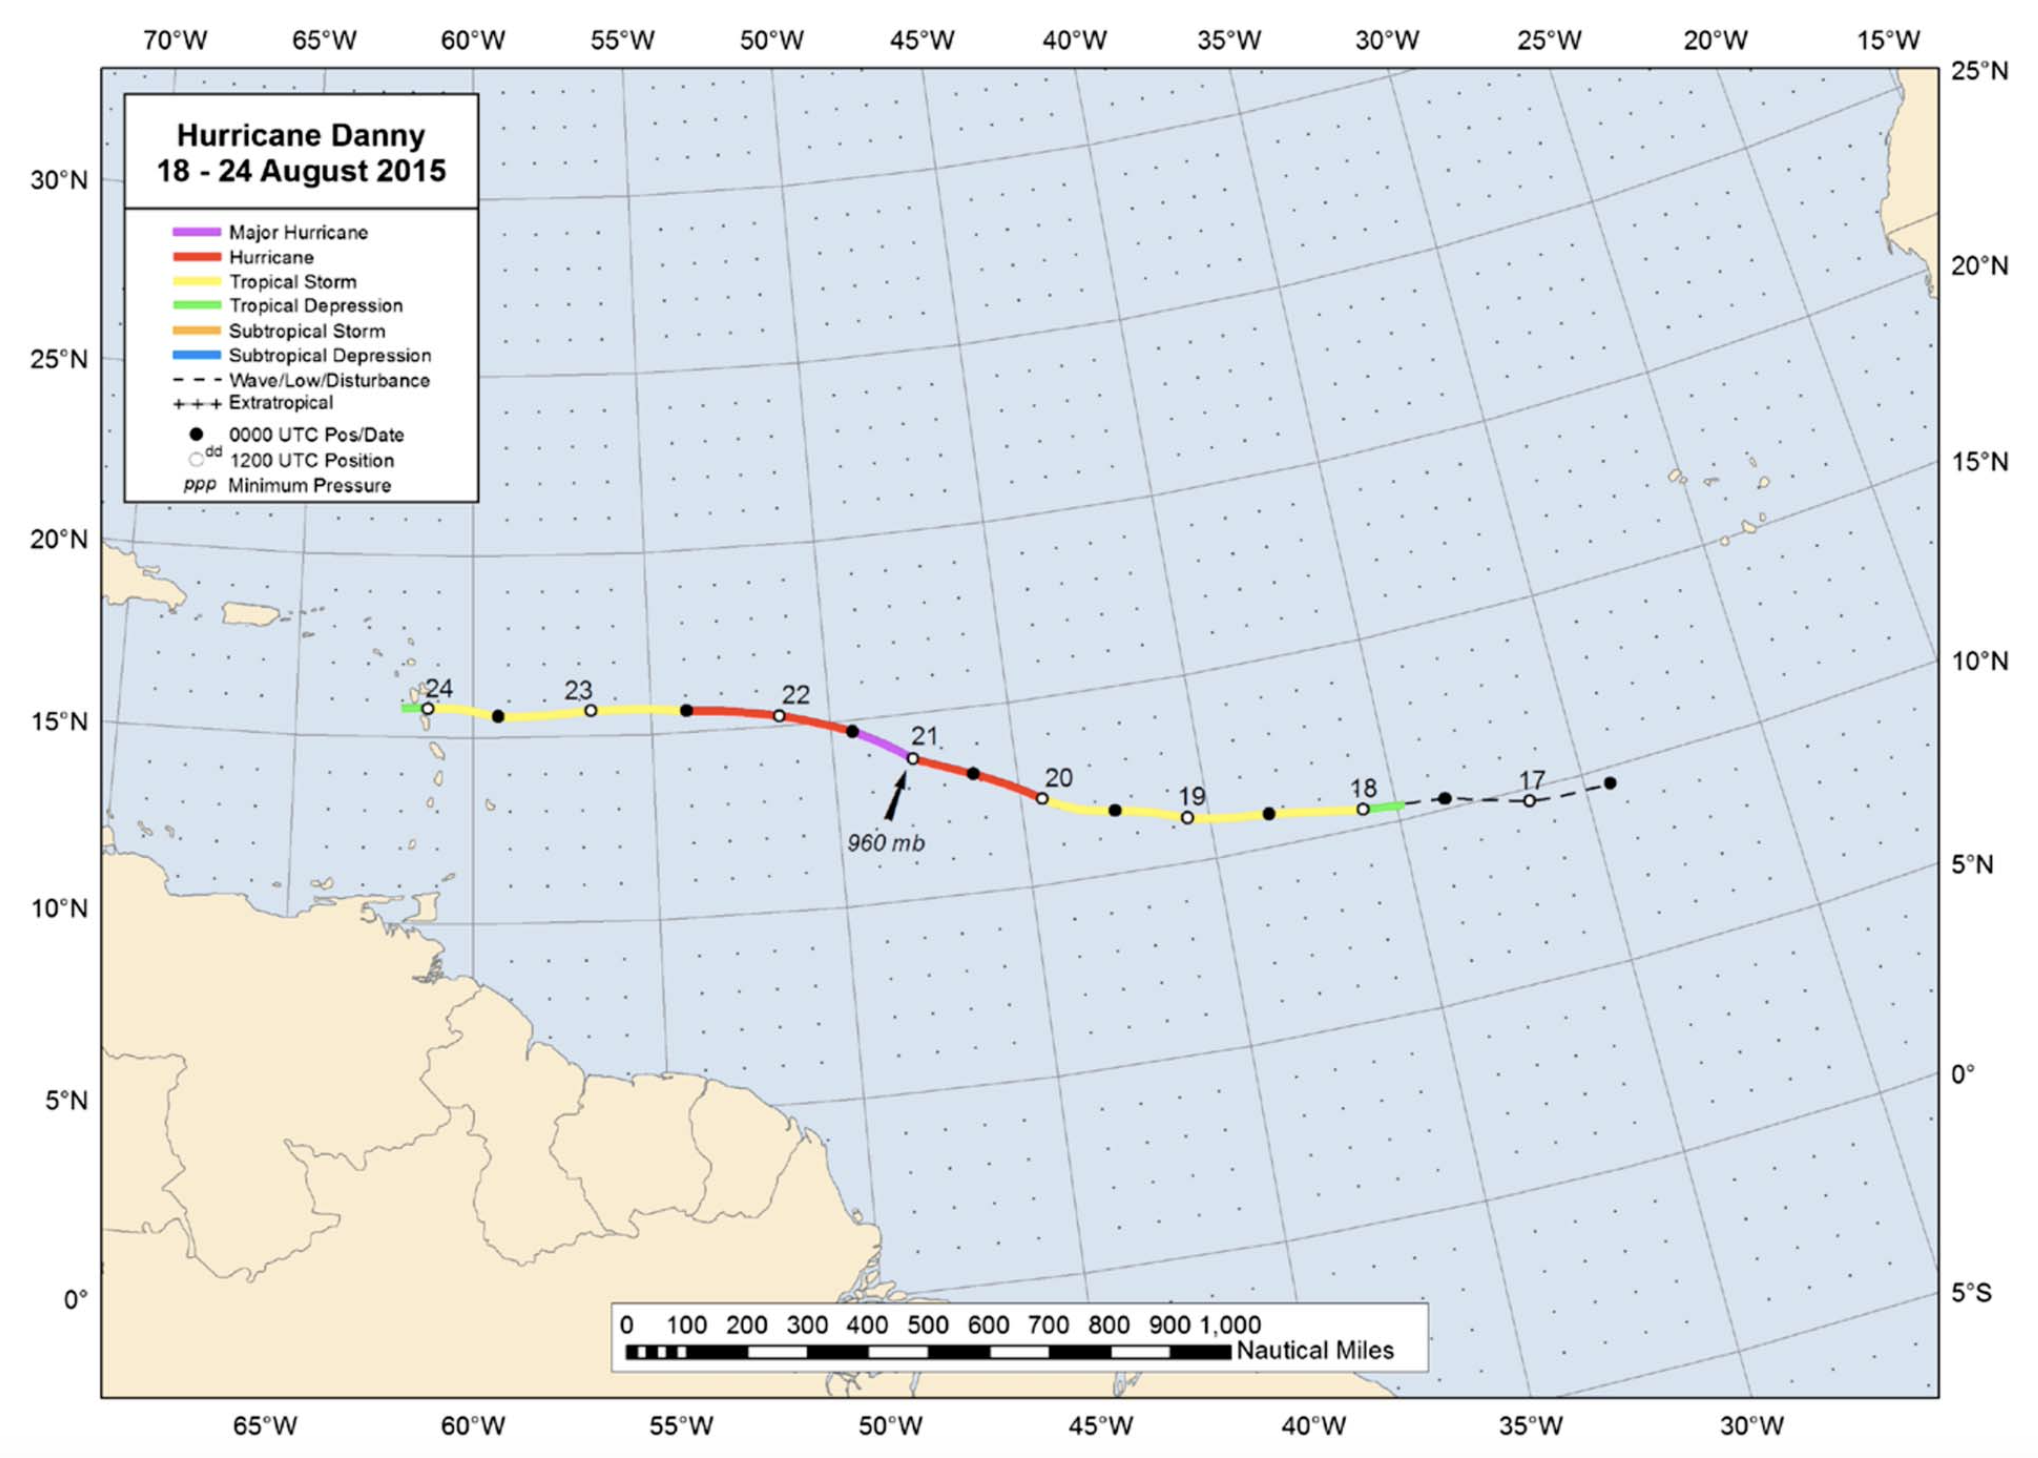
\includegraphics{figures/cyclone}}
\end{frame}
%
\begin{frame}
  \frametitle{optimal control problem}
  %
  \pause consider the following optimal control problem
  %
  \begin{subequations}
    \begin{align}
      \underset{u \in C^1}{\text{minimize}} && & J(u) = \int_0^T \|u\|_A^2 \mathrm{d}t \\
      \text{s.t.} && & \dot{x}(t) = b(x) + u(t) \\
                  && & x(0) = x_0 \\
                  && & \Phi(x(T)) = 0
    \end{align}
  \end{subequations}
  %
  \pause and discretize into
  %
  \begin{subequations}
    \begin{align}
      \underset{\{ u_k \}^N_{k = 1}}{\text{minimize}} && & J(u) = \Delta t \sum^{N}_{k = 1} \left [ u^{\top}_k A u_k \right ] \\
      \text{s.t.} && & x_{k + 1} = b(x_k) \Delta t + u_k \Delta t, \quad k \in [0, N-1]\\
                  && & x_1 = \bar{x} \\
                  && & \Phi(x_N) = 0
    \end{align}
  \end{subequations}
  %
\end{frame}
%
\begin{frame}
  \frametitle{coding example}
  CG in \texttt{Julia}, see: \href{https://github.com/jacob-roth}{\texttt{cg-pres/} repo}
\end{frame}
%
\begin{frame}
  \frametitle{coding results}
  %
  \centering \resizebox{!}{8cm}{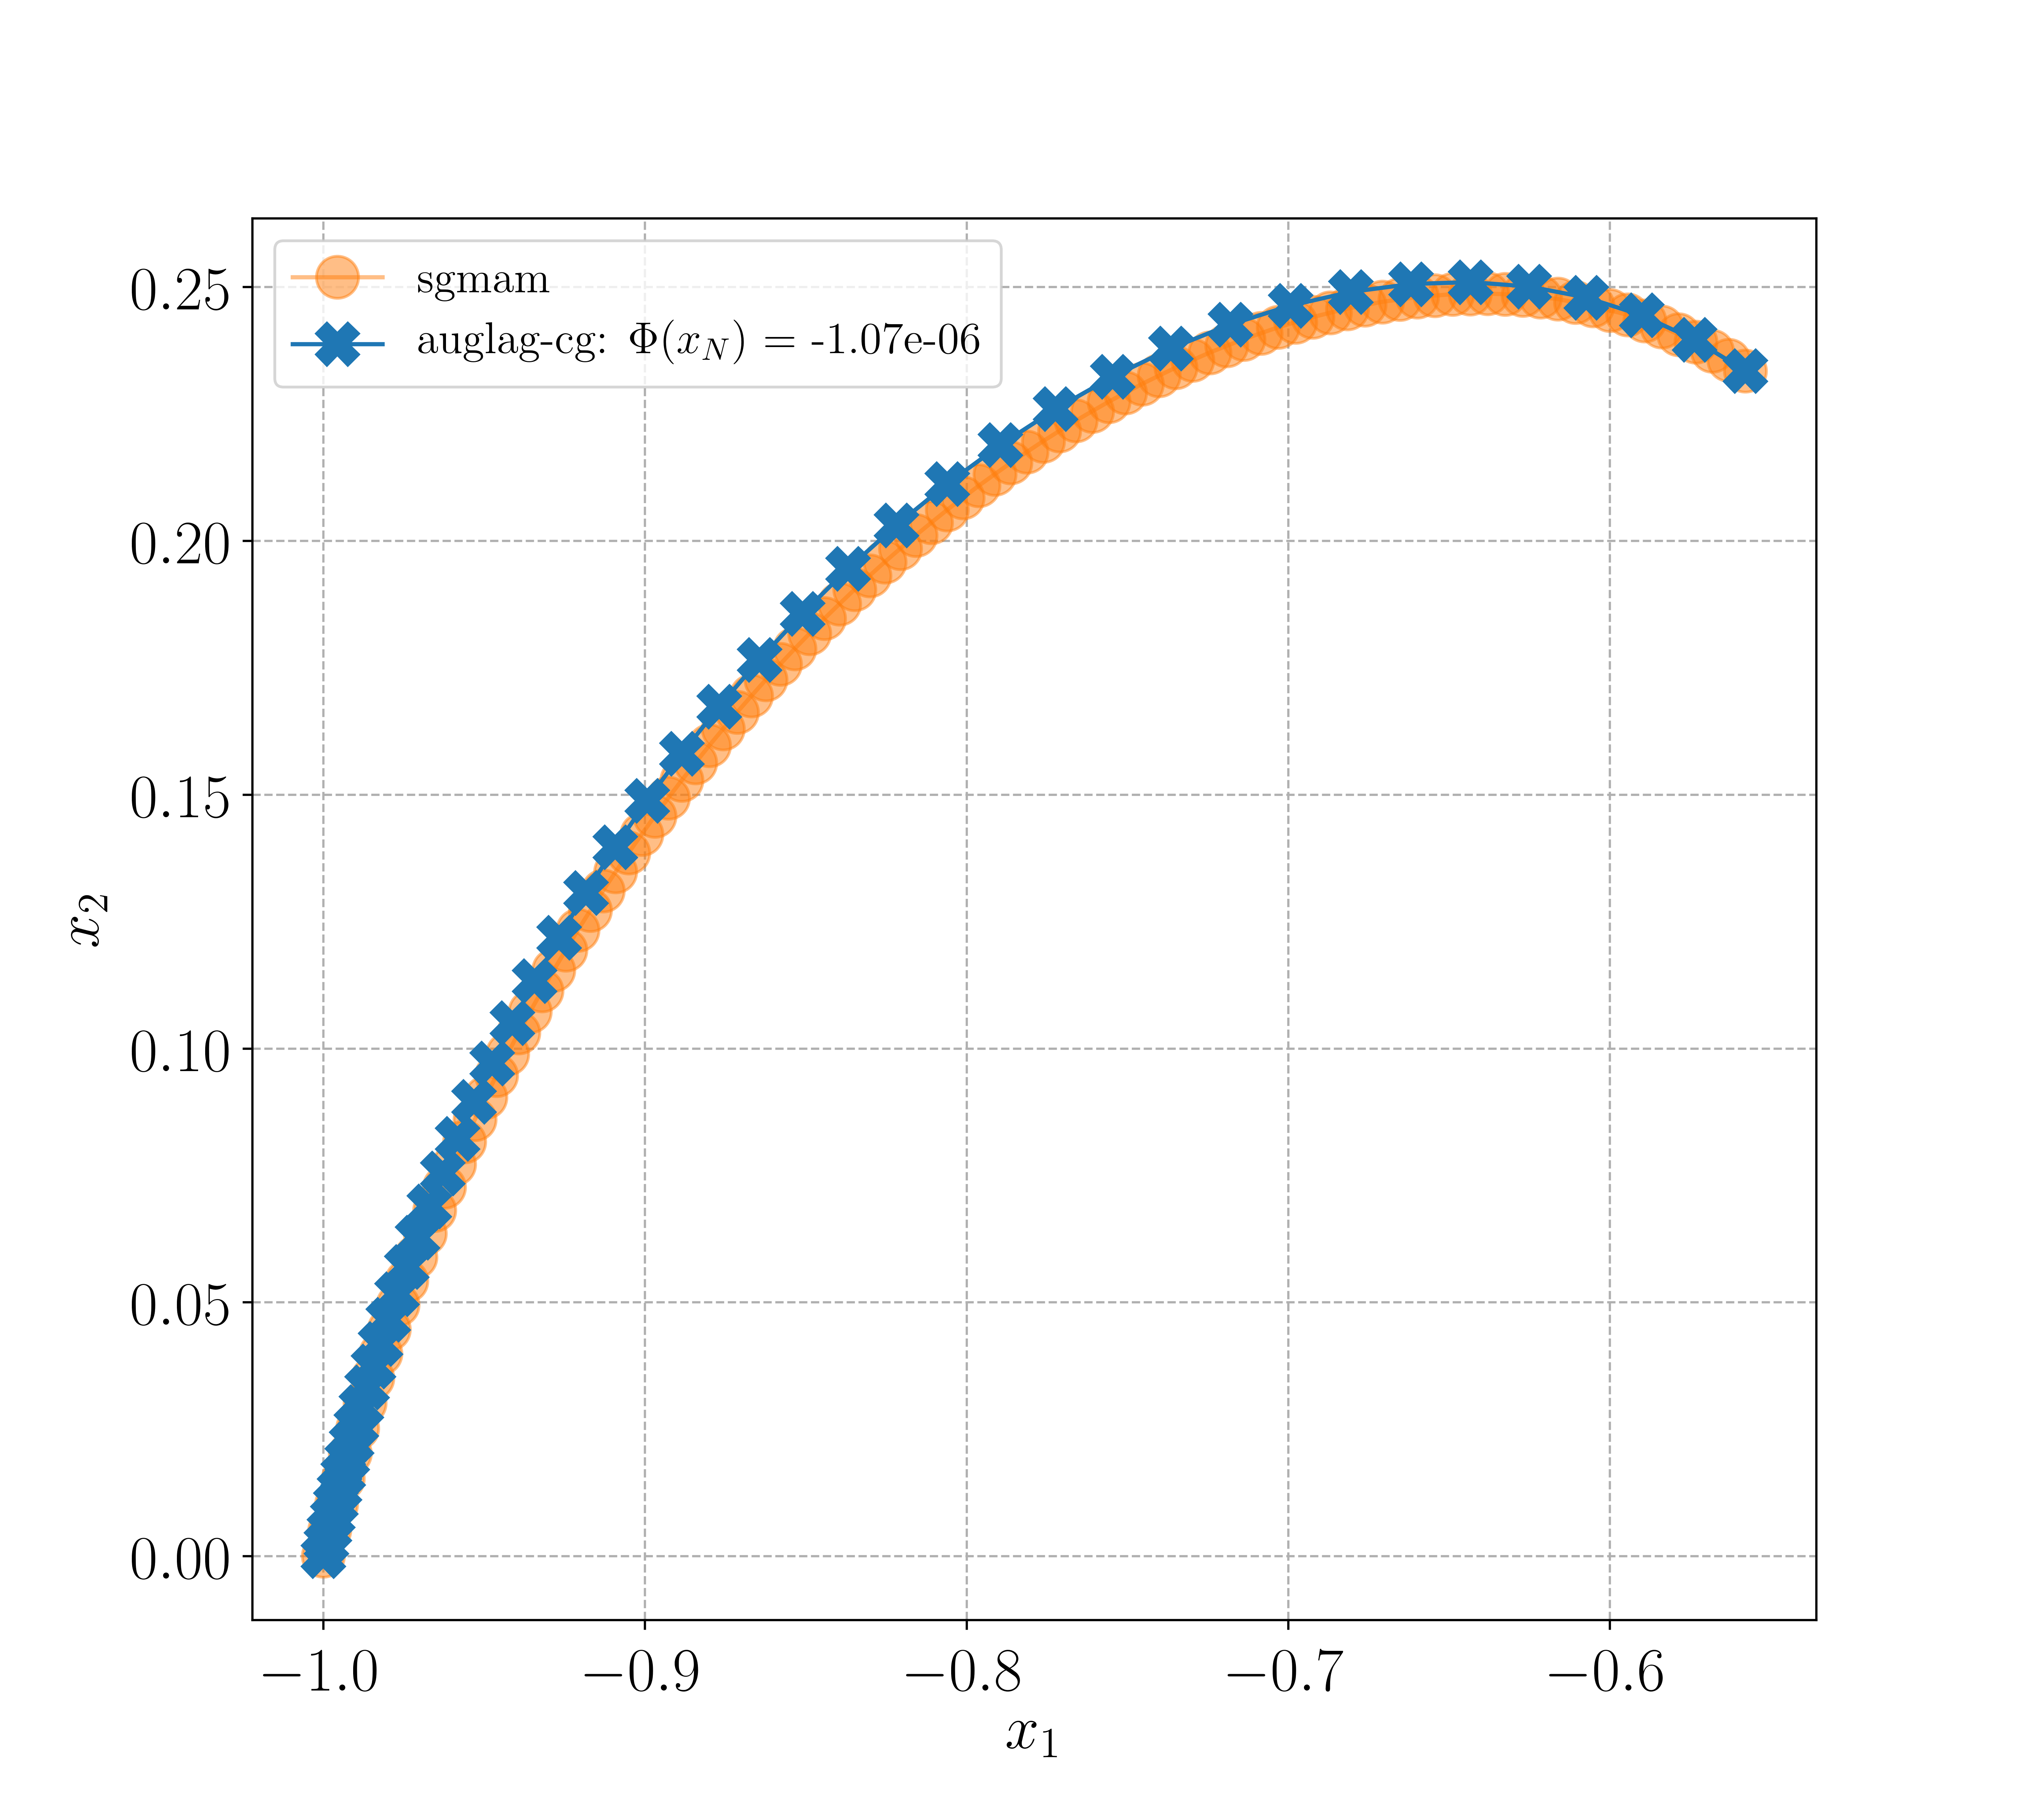
\includegraphics{figures/optimal-control}}
\end{frame}
%
%%%
%%% references
%%%
\begin{frame}[allowframebreaks]
  \frametitle{References}
  \setbeamertemplate{bibliography item}{\insertbiblabel}
  \bibliographystyle{ieeetr}
  \bibliography{refs}
\end{frame}
\end{document}

%% refs
- https://www.math.ucla.edu/~wotaoyin/math273a/slides/Lec3_gradient_descent_273a_2015_f.pdf

\begin{block}{iteration}
  at each step $k$, choose $d_k = -\nabla f(x_k)$ and $\alpha$ so that
  \begin{enumerate}
    \item $p_k = \alpha^{\star} d_k$
    \item $f(x_k + p_k) < f(x_k)$ by as much as possible
  \end{enumerate}
\end{block}

\begin{block}{general $A$ ($A \succ 0, A=A^{\top}$)}
\end{block}

\begin{frame}
  \frametitle{useful results from linear algebra}
  - diagonalizable
  - spectral theorem
  - gram-schmidt (need modified for numerics)
\end{frame}